%  LaTeX support: latex@mdpi.com
%  For support, please attach all files needed for compiling as well as the log file, and specify your operating system, LaTeX version, and LaTeX editor.

%=================================================================
\documentclass[algorithms,article,submit,pdftex,moreauthors]{Definitions/mdpi}
% For posting an early version of this manuscript as a preprint, you may use "preprints" as the journal and change "submit" to "accept". The document class line would be, e.g., \documentclass[preprints,article,accept,moreauthors,pdftex]{mdpi}. This is especially recommended for submission to arXiv, where line numbers should be removed before posting. For preprints.org, the editorial staff will make this change immediately prior to posting.

%--------------------
% Class Options:
%--------------------
%----------
% journal
%----------
% Choose between the following MDPI journals:
% acoustics, actuators, addictions, admsci, adolescents, aerospace, agriculture, agriengineering, agronomy, ai, algorithms, allergies, alloys, analytica, animals, antibiotics, antibodies, antioxidants, applbiosci, appliedchem, appliedmath, applmech, applmicrobiol, applnano, applsci, aquacj, architecture, arts, asc, asi, astronomy, atmosphere, atoms, audiolres, automation, axioms, bacteria, batteries, bdcc, behavsci, beverages, biochem, bioengineering, biologics, biology, biomass, biomechanics, biomed, biomedicines, biomedinformatics, biomimetics, biomolecules, biophysica, biosensors, biotech, birds, bloods, blsf, brainsci, breath, buildings, businesses, cancers, carbon, cardiogenetics, catalysts, cells, ceramics, challenges, chemengineering, chemistry, chemosensors, chemproc, children, chips, cimb, civileng, cleantechnol, climate, clinpract, clockssleep, cmd, coasts, coatings, colloids, colorants, commodities, compounds, computation, computers, condensedmatter, conservation, constrmater, cosmetics, covid, crops, cryptography, crystals, csmf, ctn, curroncol, currophthalmol, cyber, dairy, data, dentistry, dermato, dermatopathology, designs, diabetology, diagnostics, dietetics, digital, disabilities, diseases, diversity, dna, drones, dynamics, earth, ebj, ecologies, econometrics, economies, education, ejihpe, electricity, electrochem, electronicmat, electronics, encyclopedia, endocrines, energies, eng, engproc, ent, entomology, entropy, environments, environsciproc, epidemiologia, epigenomes, est, fermentation, fibers, fintech, fire, fishes, fluids, foods, forecasting, forensicsci, forests, foundations, fractalfract, fuels, futureinternet, futureparasites, futurepharmacol, futurephys, futuretransp, galaxies, games, gases, gastroent, gastrointestdisord, gels, genealogy, genes, geographies, geohazards, geomatics, geosciences, geotechnics, geriatrics, hazardousmatters, healthcare, hearts, hemato, heritage, highthroughput, histories, horticulturae, humanities, humans, hydrobiology, hydrogen, hydrology, hygiene, idr, ijerph, ijfs, ijgi, ijms, ijns, ijtm, ijtpp, immuno, informatics, information, infrastructures, inorganics, insects, instruments, inventions, iot, j, jal, jcdd, jcm, jcp, jcs, jdb, jeta, jfb, jfmk, jimaging, jintelligence, jlpea, jmmp, jmp, jmse, jne, jnt, jof, joitmc, jor, journalmedia, jox, jpm, jrfm, jsan, jtaer, jzbg, kidney, kidneydial, knowledge, land, languages, laws, life, liquids, literature, livers, logics, logistics, lubricants, lymphatics, machines, macromol, magnetism, magnetochemistry, make, marinedrugs, materials, materproc, mathematics, mca, measurements, medicina, medicines, medsci, membranes, merits, metabolites, metals, meteorology, methane, metrology, micro, microarrays, microbiolres, micromachines, microorganisms, microplastics, minerals, mining, modelling, molbank, molecules, mps, msf, mti, muscles, nanoenergyadv, nanomanufacturing, nanomaterials, ncrna, network, neuroglia, neurolint, neurosci, nitrogen, notspecified, nri, nursrep, nutraceuticals, nutrients, obesities, oceans, ohbm, onco, oncopathology, optics, oral, organics, organoids, osteology, oxygen, parasites, parasitologia, particles, pathogens, pathophysiology, pediatrrep, pharmaceuticals, pharmaceutics, pharmacoepidemiology, pharmacy, philosophies, photochem, photonics, phycology, physchem, physics, physiologia, plants, plasma, pollutants, polymers, polysaccharides, poultry, powders, preprints, proceedings, processes, prosthesis, proteomes, psf, psych, psychiatryint, psychoactives, publications, quantumrep, quaternary, qubs, radiation, reactions, recycling, regeneration, religions, remotesensing, reports, reprodmed, resources, rheumato, risks, robotics, ruminants, safety, sci, scipharm, seeds, sensors, separations, sexes, signals, sinusitis, skins, smartcities, sna, societies, socsci, software, soilsystems, solar, solids, sports, standards, stats, stresses, surfaces, surgeries, suschem, sustainability, symmetry, synbio, systems, taxonomy, technologies, telecom, test, textiles, thalassrep, thermo, tomography, tourismhosp, toxics, toxins, transplantology, transportation, traumacare, traumas, tropicalmed, universe, urbansci, uro, vaccines, vehicles, venereology, vetsci, vibration, viruses, vision, waste, water, wem, wevj, wind, women, world, youth, zoonoticdis

%---------
% article
%---------
% The default type of manuscript is "article", but can be replaced by:
% abstract, addendum, article, book, bookreview, briefreport, casereport, comment, commentary, communication, conferenceproceedings, correction, conferencereport, entry, expressionofconcern, extendedabstract, datadescriptor, editorial, essay, erratum, hypothesis, interestingimage, obituary, opinion, projectreport, reply, retraction, review, perspective, protocol, shortnote, studyprotocol, systematicreview, supfile, technicalnote, viewpoint, guidelines, registeredreport, tutorial
% supfile = supplementary materials

%----------
% submit
%----------
% The class option "submit" will be changed to "accept" by the Editorial Office when the paper is accepted. This will only make changes to the frontpage (e.g., the logo of the journal will get visible), the headings, and the copyright information. Also, line numbering will be removed. Journal info and pagination for accepted papers will also be assigned by the Editorial Office.

%------------------
% moreauthors
%------------------
% If there is only one author the class option oneauthor should be used. Otherwise use the class option moreauthors.

%---------
% pdftex
%---------
% The option pdftex is for use with pdfLaTeX. If eps figures are used, remove the option pdftex and use LaTeX and dvi2pdf.
\usepackage{gensymb}
\usepackage{amsmath}
\usepackage{accents}
\usepackage{multirow}
\usepackage{xspace}
\usepackage{subcaption}
\DeclareRobustCommand{\w}{\mbox{\large\ensuremath{\mathsf{w}}}}
\DeclareRobustCommand{\A}{\mbox{\large\ensuremath{\mathsf{A}}}}
\DeclareRobustCommand{\B}{\mbox{\large\ensuremath{\mathsf{B}}}}
\DeclareRobustCommand{\C}{\mbox{\large\ensuremath{\mathsf{C}}}}
\DeclareRobustCommand{\Dev}{\mbox{\Large\ensuremath{\mathsf{s}}}}
\DeclareRobustCommand{\Sig}{\mbox{\Large\ensuremath{\sigma}}}
\DeclareRobustCommand{\dotp}{\boldsymbol{\cdot}}
\DeclareRobustCommand{\ccirc}{\kern0.5ex\vcenter{\hbox{$\scriptstyle\circ$}}\kern0.5ex}
\DeclareRobustCommand{\e}[1]{{\rm e}^{#1}}
\DeclareRobustCommand{\lay}[1]{^{(#1)}}
\DeclareRobustCommand{\mdot}[1]{\accentset{\mbox{\bfseries .}}{#1}}
\DeclareRobustCommand{\ie}{\emph{i.e.}\@\xspace}
\DeclareRobustCommand{\eal}{et \emph{al.}\@\xspace}
\DeclareRobustCommand{\eg}{e.g.,\@\xspace}
\DeclareRobustCommand{\MSE}{\text{E}_\text{MS}}
\DeclareRobustCommand{\RMSE}{\text{E}_\text{RMS}}
\DeclareRobustCommand{\MARE}{\text{E}_\text{MAR}}
\DeclareRobustCommand{\R}{\text{R}}
\DeclareRobustCommand{\ps}{\text{s}^{-1}}
\DeclareRobustCommand{\mr}[2]{\multirow{#1}{*}{#2}}
\DeclareRobustCommand{\MPa}{\text{MPa}}

%=================================================================
% MDPI internal commands
\firstpage{1}
\makeatletter
\setcounter{page}{\@firstpage}
\makeatother
\pubvolume{1}
\issuenum{1}
\articlenumber{0}
\pubyear{2022}
\copyrightyear{2022}
%\externaleditor{Academic Editor: Firstname Lastname}
\datereceived{}
%\daterevised{} % Only for the journal Acoustics
\dateaccepted{}
\datepublished{}
%\datecorrected{} % Corrected papers include a "Corrected: XXX" date in the original paper.
%\dateretracted{} % Corrected papers include a "Retracted: XXX" date in the original paper.
\hreflink{https://doi.org/} % If needed use \linebreak
%\doinum{}
%------------------------------------------------------------------
% The following line should be uncommented if the LaTeX file is uploaded to arXiv.org
%\pdfoutput=1

%=================================================================
% Add packages and commands here. The following packages are loaded in our class file: fontenc, inputenc, calc, indentfirst, fancyhdr, graphicx, epstopdf, lastpage, ifthen, lineno, float, amsmath, setspace, enumitem, mathpazo, booktabs, titlesec, etoolbox, tabto, xcolor, soul, multirow, microtype, tikz, totcount, changepage, attrib, upgreek, cleveref, amsthm, hyphenat, natbib, hyperref, footmisc, url, geometry, newfloat, caption

%=================================================================
%% Please use the following mathematics environments: Theorem, Lemma, Corollary, Proposition, Characterization, Property, Problem, Example, ExamplesandDefinitions, Hypothesis, Remark, Definition, Notation, Assumption
%% For proofs, please use the proof environment (the amsthm package is loaded by the MDPI class).

%=================================================================
% Full title of the paper (Capitalized)
\Title{Development and Implementation of an ANN based flow law for Numerical Simulations of Thermo-mechanical Processes at High Temperatures in FEM Software}

% MDPI internal command: Title for citation in the left column
\TitleCitation{Development and Implementation of an ANN based flow law for Numerical Simulations Thermo-mechanical Processes at High Temperatures in FEM Software}

% Author Orchid ID: enter ID or remove command
\newcommand{\orcidauthorA}{0000-0001-7367-5453} % Add \orcidA{} behind the author's name
%\newcommand{\orcidauthorB}{0000-0000-0000-000X} % Add \orcidB{} behind the author's name

% Authors, for the paper (add full first names)
\Author{Olivier Pantalé \orcidA{}}

%\longauthorlist{yes}

% MDPI internal command: Authors, for metadata in PDF
\AuthorNames{Olivier Pantalé}

% MDPI internal command: Authors, for citation in the left column
\AuthorCitation{Pantalé, O.}
% If this is a Chicago style journal: Lastname, Firstname, Firstname Lastname, and Firstname Lastname.

% Affiliations / Addresses (Add [XX] after \address if there is only one affiliation.)
\address[1]{Laboratoire Génie de Production, Institut National Polytechnique/Ecole Nationale d'Ingénieurs de Tarbes, Université de Toulouse, 47 Av d'Azereix, F-65016, Tarbes, France}

% Contact information of the corresponding author
\corres{Correspondence: Olivier.Pantale@enit.fr; Tel.: +33-562442933}

% Current address and/or shared authorship

% The commands \thirdnote{} till \eighthnote{} are available for further notes

%\simplesumm{} % Simple summary

%\conference{} % An extended version of a conference paper

% Abstract (Do not insert blank lines, i.e. \\)
\abstract{Numerical methods based on Finite Element (FE) have proven their efficiency for many years in the thermomechanical simulation of forming processes.
Nevertheless, the application of these methods to new materials requires the identification and implementation of constitutive and flow laws within FE codes which sometimes pose problems, in particular because of the very strongly non-linear character of the behavior of these materials.
Computational techniques based on Machine Learning and Artificial Neural Networks are becoming more and more important in the development of these models and help the FE codes to integrate more complex behavior.
In this paper, we present the development, implementation and use of an Artificial Neural Network (ANN) based flow law for a GrC15 alloy under high temperature thermomechanical sollicitations.
The flow law modeling by ANN shows a significant superiority in terms of model prediction quality compared to classical approaches based on widely used Johnson-Cook or Arrhenius models.
Once the ANN parameters have been identified on the base of experiments, the implementation of this flow law in a Finite Element code shows promising results in terms of solution quality and respect of the material behavior.}

% Keywords
\keyword{ANN flow law; Constitutive behavior; Radial Return algorithm; Numerical implementation; VUHARD ; GrC15; Abaqus Explicit}

% The fields PACS, MSC, and JEL may be left empty or commented out if not applicable
%\PACS{J0101}
%\MSC{}
%\JEL{}

%%%%%%%%%%%%%%%%%%%%%%%%%%%%%%%%%%%%%%%%%%
% Only for the journal Diversity
%\LSID{\url{http://}}

%%%%%%%%%%%%%%%%%%%%%%%%%%%%%%%%%%%%%%%%%%
% Only for the journal Applied Sciences
%\featuredapplication{Authors are encouraged to provide a concise description of the specific application or a potential application of the work. This section is not mandatory.}
%%%%%%%%%%%%%%%%%%%%%%%%%%%%%%%%%%%%%%%%%%

%%%%%%%%%%%%%%%%%%%%%%%%%%%%%%%%%%%%%%%%%%
% Only for the journal Data
%\dataset{DOI number or link to the deposited data set if the data set is published separately. If the data set shall be published as a supplement to this paper, this field will be filled by the journal editors. In this case, please submit the data set as a supplement.}
%\datasetlicense{License under which the data set is made available (CC0, CC-BY, CC-BY-SA, CC-BY-NC, etc.)}

%%%%%%%%%%%%%%%%%%%%%%%%%%%%%%%%%%%%%%%%%%
% Only for the journal Toxins
%\keycontribution{The breakthroughs or highlights of the manuscript. Authors can write one or two sentences to describe the most important part of the paper.}

%%%%%%%%%%%%%%%%%%%%%%%%%%%%%%%%%%%%%%%%%%
% Only for the journal Encyclopedia
%\encyclopediadef{For entry manuscripts only: please provide a brief overview of the entry title instead of an abstract.}

%%%%%%%%%%%%%%%%%%%%%%%%%%%%%%%%%%%%%%%%%%
% Only for the journal Advances in Respiratory Medicine
%\addhighlights{yes}
%\renewcommand{\addhighlights}{%

%\noindent This is an obligatory section in “Advances in Respiratory Medicine”, whose goal is to increase the discoverability and readability of the article via search engines and other scholars. Highlights should not be a copy of the abstract, but a simple text allowing the reader to quickly and simplified find out what the article is about and what can be cited from it. Each of these parts should be devoted up to 2~bullet points.\vspace{3pt}\\
%\textbf{What are the main findings?}
% \begin{itemize}[labelsep=2.5mm,topsep=-3pt]
% \item First bullet.
% \item Second bullet.
% \end{itemize}\vspace{3pt}
%\textbf{What is the implication of the main finding?}
% \begin{itemize}[labelsep=2.5mm,topsep=-3pt]
% \item First bullet.
% \item Second bullet.
% \end{itemize}
%}

%%%%%%%%%%%%%%%%%%%%%%%%%%%%%%%%%%%%%%%%%%
\begin{document}

%%%%%%%%%%%%%%%%%%%%%%%%%%%%%%%%%%%%%%%%%%%
%\setcounter{section}{-1} %% Remove this when starting to work on the template.
%\section{How to Use this Template}
%
%The template details the sections that can be used in a manuscript. Note that the order and names of article sections may differ from the requirements of the journal (e.g., the positioning of the Materials and Methods section). Please check the instructions on the authors' page of the journal to verify the correct order and names. For any questions, please contact the editorial office of the journal or support@mdpi.com. For LaTeX-related questions please contact latex@mdpi.com.%\endnote{This is an endnote.} % To use endnotes, please un-comment \printendnotes below (before References). Only journal Laws uses \footnote.
%
%% The order of the section titles is different for some journals. Please refer to the "Instructions for Authors” on the journal homepage.
%

%------------------------------------------------------------------------------------
\section{Introduction}\label{sec:Introduction}
%------------------------------------------------------------------------------------

Numerical methods for simulating the behavior of structures subjected to high thermomechanical loads, as in the case of high-temperature forming of metallic materials, are generally based on the use of commercial Finite Element (FE) codes such as Abaqus or laboratory codes such as DynELA \cite{Pantale-2004}.
These FE codes are based on two types of equations: conservation equations and constitutive equations.
If the first equations are generally well established on the basis of physics and mechanics, it is not the same for the second type of equations: the constitutive equations.
Thus, in a general way, the conservation equations concern the fundamental principles of physics such as the mass conservation law, the momentum law (fundamental equation) and the energy law (declined in the form of the first and second principles of thermodynamics).
By themselves, these laws are not sufficient to describe the behavior of a material or a structure subjected to thermomechanical solicitations, because the nature of the material's behavior, generally translated by means of the behavior laws, is not included in the system previously proposed.
Therefore, for each type of material, it is necessary to define behavior laws whose formulation is based on observation, in order to describe the behavior of this material under external forces.
The quality and the accuracy of the results of any numerical simulation depend on the choice of these behavior laws and on the ability of the user to identify the coefficients of these behavior laws for a given material by performing experiments under conditions close to those encountered during the real stress of the structure in service that one wishes to design.
Depending on the nature of the solicitations, these tests are based on quasi-static or dynamic tensile or compression tests, tests on thermomechanical simulators such as Gleeble \cite{Lin-2009} or impact tests using gas launchers or Hopkinson bars \cite{Kolsky-1949}.

In the context of thermomechanical simulation of forming processes, these behavior laws define the dependence of the flow stress of the material $\sigma^y$ as a function of the three input variables which are the plastic strain $\varepsilon^p$, the strain rate $\mdot\varepsilon$ and the temperature $T$ of the material, so that the general form of the flow law can be written with the following expression:
\begin{equation}
\sigma^y = f\left(\varepsilon^p,\mdot\varepsilon,T\right)\label{eq:GenFlow}
\end{equation}

These laws, due to the nature of materials and the phenomena involved (work hardening, movement of dislocations, structural hardening, phase transformations, ...) are highly non-linear and their validity is restricted to a certain range of strains $\varepsilon$, strain rates $\mdot\varepsilon$ and temperatures $T$.
From the observations made, we can define two main classes of behavior laws: the flow laws based on physics and the empirical flow laws.
From the mechanics of continuous media and experimental tests and depending on the nature of the materials used, a number of flow models have been developed in the past, including: the Johnson-Cook flow law \cite{Johnson-1983}, the Zerilli Armstrong flow law \cite{Zerilli-1987} and their respective derived forms \cite{Rule-1998, Lin-2011, Li-2013, Zhang-2015, Zhou-2020}, the Hansel-Spittle \cite{Hensel-1978} or the Arrhenius \cite{Jonas-1969} flow laws, to name only a few of the most widely used in the context of the metal forming processes at high temperature.
As an example, and because it is widely used in numerical simulation of metal forming processes, the equation that describes the Johnson-Cook flow law \cite{Johnson-1983} is given as follows:
\begin{equation}
\sigma^y=\left(A+B\varepsilon^{p^{n}}\right) \left[1+C\ln\left(\frac{\mdot\varepsilon}{\mdot\varepsilon_0}\right)\right] \left[1-\left(\frac{T-T_0}{T_m-T_0}\right)^{m}\right],\label{eq:Johnson-Cook}
\end{equation}
where $A$ is the initial elastic limit of the material, $B$ is the strain hardening coefficient, $n$ is the strain hardening exponent, $C$ and $m$ are the material constants that describe the strain rate hardening coefficient and the thermal softening coefficient, respectively.

Once the choice has been made concerning the type of flow law to be used for a given material, it is then necessary, from a set of experimental tests carried out in the laboratory under conditions close to those of the structure in service, to identify the parameters of these flow laws by machine learning methods based on approaches of minimization of the calculated experiment.
Therefore, the use of the Johnson-Cook flow law defined by Equation (\ref{eq:Johnson-Cook}) require the identification of $5$ material parameters.

The main problem that the researchers are confronted with after the phase of realization of the experimental tests concerns the choice of the flow law to use according to the observations made on these test results.
This choice of flow law is also restricted by the nature of the FE code used and the availability of such flow laws.
Thus, a user of the Abaqus FE code, will turn more particularly to a Johnson-Cook \cite{Johnson-1983} flow law insofar as it is natively implemented in this software.
The choice of another form of flow law, Zerilli-Armstrong, or Arrhenius for example, obliges the user to program himself the computation of the flow stress $\sigma^y$ of the material by means of a VUMAT subroutine in FORTRAN 77 as proposed by Gao \eal \cite{Gao-2007-FRT}, Ming \eal \cite{Ming-2018} for a Johnson-Cook flow law or Liang \eal \cite{Liang-2022} for an Arrhenius type flow law with the following expression:
\begin{equation}
\sigma^y = \frac{1}{\alpha(\varepsilon)} \ln\left\{\left(\frac{Z(\varepsilon)}{A(\varepsilon)}\right)^{1/n(\varepsilon)} + \sqrt{1 + \left(\frac{Z(\varepsilon)}{A(\varepsilon)}\right)^{2/n(\varepsilon)}}\right\}
\label{eq:ArDef}
\end{equation}
with:
\begin{equation}
Z(\varepsilon) = \mdot\varepsilon \exp{\left(\frac{Q(\varepsilon)}{RT}\right)}, \label{eq:ArZ}
\end{equation}
where $Z$ is the Zenner-Hollomon parameter \cite{Zener-1944}, $Q(\varepsilon)$ is the apparent activation energy ($\text{J~mol}^{-1}$), $R$ is the universal gas constant ($8.314~\text{J~mol}^{-1} \text{K}^{-1}$).
$Q(\varepsilon)$, $A(\varepsilon)$, $\alpha(\varepsilon)$ and $n(\varepsilon)$ are expressed as a function of the strain $\varepsilon$ by means of polynomial functions of degree $m$ (varying from $1$ to $9$), which leads to the identification of up-to $36$ material parameters.

The implementation of the flow law as a VUMAT FORTRAN subroutine requires the computation of the derivatives  $\partial\sigma^y/\partial\varepsilon^p$, $\partial\sigma^y/\partial\mdot\varepsilon$ and $\partial\sigma^y/\partial T$ of the flow stress $\sigma^y$ which can quickly become relatively complex as the complexity of the flow law increases, \ie the relative complexity of the Arrhenius flow law defined by Equations (\ref{eq:ArDef}) and (\ref{eq:ArZ}), with regard to the relative simplicity of the Johnson-Cook defined by Equation (\ref{eq:Johnson-Cook}), one can refer to the work proposed by Liang \eal \cite{Liang-2022} for details concerning this implementation using the Safe version of the Newton-Raphson method proposed by Ming \eal \cite{Ming-2018}.
The choice of the flow law to use for a given problem, is therefore doubly guided by the nature of the behavior of the material on the one hand, but a more important aspect is the list of flow laws implemented natively in the FE code we plan to use for the numerical simulation.
At this time, there is not yet a flow law generic enough to cover a wide range of material behavior that is simple to implement and use.

As we have seen in the previous paragraph, the choice of the flow law to use is generally guided mainly by the list of flow laws available in the Finite Element code used, and very often this choice is made at the expense of the quality of the model.
For example, Zhou \eal \cite{Zhou-2020}, proposed the identification of the flow law of a GCr15 alloy for a continuous casting bloom with heavy reduction application as introduced by Ji \eal \cite{Ji-2018} who have performed compression tests on this material.
In their study, Ji \eal \cite{Ji-2018} performed compression tests on GCr15 cylinders in a temperature range of $750~\celsius$ to $1300~\celsius$ in $50~\celsius$ steps, strain rates of $0.001~\ps$,  $0.01~\ps$ and $0.1~\ps$ and strains up-to $0.7$.
The results of these compression tests, plotted in Figure \ref{fig:Zhou-OriginalData}, show a decrease in flow stress $\sigma^y$ with respect to an increase of the temperature $T$ and a increase of $\sigma^y$ with respect to an increase of the strain rate $\mdot\varepsilon$, as in most metallic materials.
\begin{figure}[!ht]
\centering
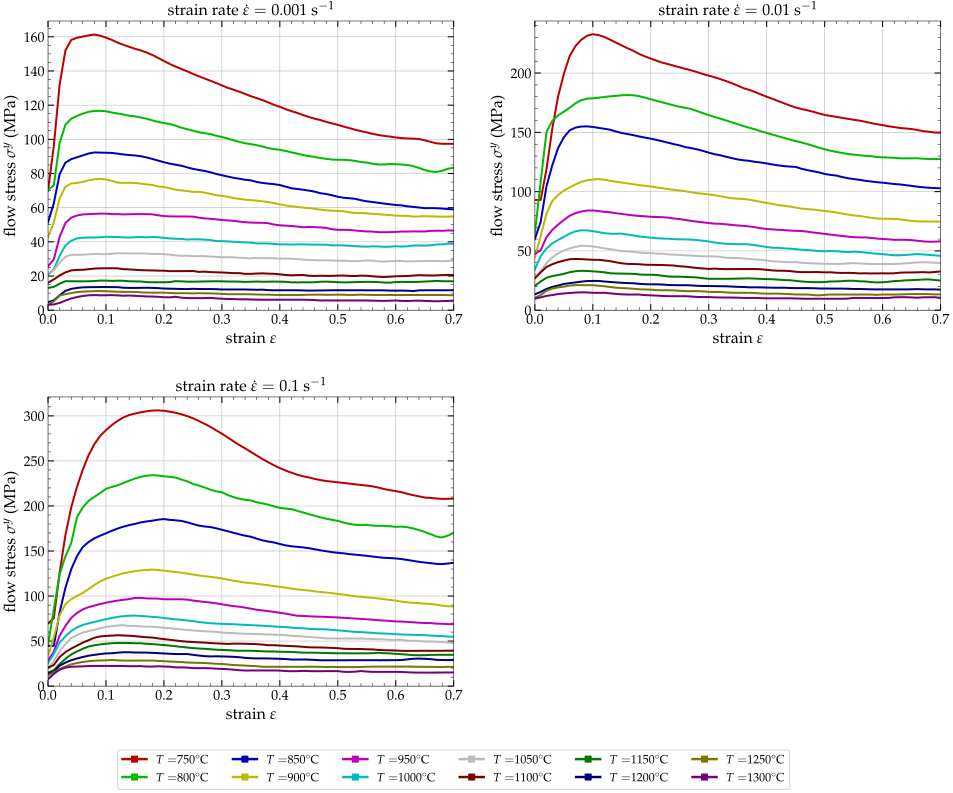
\includegraphics[width=0.9\columnwidth]{Figures/Zhou-OriginalData}
\caption{Original Data.}
\label{fig:Zhou-OriginalData}
\end{figure}
The evolution of the flow stress as a function of the plastic deformation shows the presence of a dynamic recrystallization (DRX) phenomenon within the material.
This phenomenon is an additional non-linearity of this type of material compared to other materials, mainly due to high temperatures and low strain rates, which should be taken into account when describing the material behavior.
As stated in the publication of Zhou \eal \cite{Zhou-2020}, depending on the flow model used: Johnson-Cook, Modified Zerilli-Armstrong, Arrhenius or new Modified Johnson-Cook, the fidelity of taking into account the real behavior varies widely with the complexity of the flow model which includes between $5$ parameters for the Johnson-Cook model, and $16$ parameters for the Arrhenius model.
Thus, and for the input data provides by Ji \eal \cite{Ji-2018}, the two most common models: Johnson-Cook and Zerilli-Armstrong do not correctly describe the material behavior.
Only the modified Johnson-Cook and Arrhenius models are able to describe correctly the behavior of the material during the compression process.
Unfortunately, and this is not part of their study, if these last two models are satisfactory from a theoretical point of view, from a practical point of view for the user of a FE code such as Abaqus, it will be necessary to carry out a numerical implementation in a FORTRAN 77 VUMAT subroutine of the modified Johnson-Cook flow law or the Arrhenius law as carried out by few authors \cite{Liang-2022, Gao-2007-FRT, Ming-2018} in order to be able to use these laws for numerical simulation.
This requires a certain expertise in the development and implementation of flow laws, which is not available to all users of the Abaqus FE code.

From this observation, and from the necessity to select a flow law for a given type of material, then to identify the parameters of this flow law according to experimental tests, and finally to implement this flow law in the form of a user subroutine in FORTRAN in the Abaqus FE code, we have recently proposed in Pantalé \eal \cite{Pantale-2021} an alternative approach based on the ability of Artificial Neural Networks (ANNs) to behave as universal approximators as reported by Minsky \eal \cite{Minsky-1969} and Hornik \eal \cite{Hornik-1989}.
In fact, Artificial Neural Networks can solve problems that are difficult to conceptualize using traditional computational methods.
Unlike a classical approach based on a regression method, an ANN does not need to know the mathematical form of the model it seeks to reproduce, hence we do not need anymore to postulate the mathematical form of the constitutive equation to use it in a FE simulation using this kind of approach.

The implementation of ANNs for plasticity in thermomechanics has been studied and a review of the literature can be found for example in Gorji \eal \cite{Gorji-2020} concerning the use of recurrent neural networks, in Jamli \eal \cite{Jamli-2019-SNN} concerning their application in finite element analysis of metal forming processes, or in Jiao \eal \cite{Jiao-2020} concerning the applicability to meta-materials and their characterization.
A distinction must be made between ANN-based flow models (the focus of this study) and ANN-based constitutive models.
Both approaches have been studied by many researchers during the last thirty years.
Ghaboussi \cite{Ghaboussi-1991} proposed an ANN-based constitutive model for concrete under monotonic biaxial loading and cyclic uniaxial loading.
They extended their work by introducing adaptive and autoprogressive networks in \cite{Ghaboussi-1998, Ghaboussi-1998-NNA} where the architecture of the network evolves during the learning phase to better learn the complex stress-strain behavior of the materials using a global load-deflection response where the evaluation of the flow stress of the material computed by the ANN is combined with a Radial-Return algorithm.
Lin \eal \cite{Lin-2008} proposed an ANN to predict the flow stress of 42CrMo4 steel in hot compression tests on a Gleeble thermomechanical device and showed a very good correlation between the experimental results and the model predictions.
Ashtiani \eal \cite{Ashtiani-2016} compared the predictive capabilities of an ANN versus an analytical model for Johnson-Cook, Arrhenius, and strain-compensated Arrhenius laws and concluded that the neural network had better efficiency and accuracy in predicting the hot behavior of Al-Cu-Mg-Pb alloy.

The underlying idea proposed in or approach, is to implement a flow law described by a trained ANN in the form of a FORTRAN 77 subroutine in the Abaqus FE code.
This ANN was previously trained from the data extracted from mechanical tests of the material and can directly define the value of the flow stress $\sigma^y$ as a function of the plastic strain $\varepsilon^p$, the strain rate $\mdot\varepsilon$ and the temperature $T$.
After a training phase based on the use of the Python library Tensorflow \cite{Abadi-2016, Mattmann-2020}, the weights and biases of the trained neural network are transcoded into a subroutine in FORTRAN 77 which is compiled and linked with the libraries of the Abaqus FE code in order to include the behavior of the material by allowing the computation of the flow stress $\sigma^y$ as a function of $\varepsilon^p$, $\mdot\varepsilon$ and $T$, and of its three derivatives $\partial\sigma^y/\partial\varepsilon^p$, $\partial\sigma^y/\partial\mdot\varepsilon$ and $\partial\sigma^y/\partial T$.

The structure of this paper is as follows.
Section \ref{sec:Training} deals with the presentation of a Neural Network based flow law and its training from the data proposed by Ji \eal \cite{Ji-2018} and reported in Figure \ref{fig:Zhou-OriginalData}.
The comparison of several neural network architectures regarding accuracy and implementation complexity will be presented and compared.
In Section \ref{sec:Use}, we will present the transposition of this neural network into a FORTRAN 77 subroutine for the Abaqus FE code.
Validation is based on the numerical simulation Abaqus Explicit FE code of a compression test in the same configuration as the one proposed by Ji \eal \cite{Ji-2018} using four different ANN flow laws.
Finally, a conclusion and perspective Section will conclude this paper.

%------------------------------------------------------------------------------------
\section{Training of the ANN flow law}\label{sec:Training}
%------------------------------------------------------------------------------------

In this section, we briefly recall, as an introduction, some basic principles of Artificial Neural Networks that are relevant to this work.
The global architecture chosen to model the behavior of a material is based on a multi-layer feed-forward ANN which as proposed by Hornik \eal \cite{Hornik-1989} can be used as a universal approximator.
The architecture retained for this study concerns a neural network with two hidden layers containing a variable number of neurons on these two layers, $3$ input nodes corresponding to the plastic strain $\varepsilon^p$, the strain rate $\mdot\varepsilon$ and the temperature $T$ respectively and a single output node for the flow stress $\sigma^y$ of the material.
Figure \ref{fig:ANN-scheme} shows a graphical representation of the global architecture of this neural network.
\begin{figure}[!ht]
\centering
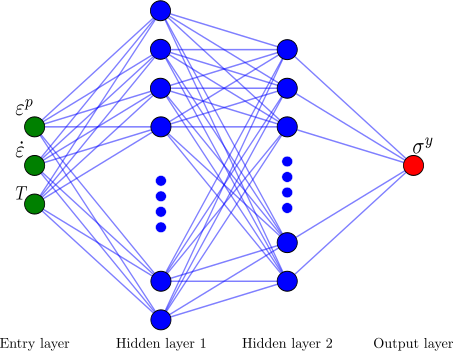
\includegraphics[width=0.7\columnwidth]{Figures/ANN-scheme-2HL}
\caption{Global structure of the ANN flow law with two hidden layers, 3 input neurons ($\varepsilon^p$, $\mdot\varepsilon$, $T$) and one output neuron $\sigma^y$.}
\label{fig:ANN-scheme}
\end{figure}
The choice of the number of neurons in the two hidden layers is free, but must be reasonable.
Indeed, the more neurons the network contains, the more it will be able to reproduce faithfully the training data, but the less it will be able to generalize to new data (the classical problem of overlearning of neural networks).
Moreover, the more neurons it contains, the more complex its mathematical structure will be, and the more computation time it will require to propagate the data inside of it within the routine included in the FE code.
It is therefore necessary to respect a balance between the capacity of the network to minimize errors during the learning phase, its complexity and the computing CPU time once it is transcribed into the FE code.

%------------------------------------------------------------------------------------
\subsection{Neural Network governing equations}\label{sec:ANN-equations}
%------------------------------------------------------------------------------------

According to Figure \ref{fig:ANN-scheme}, the proposed neural network has $3$ inputs (referred as the input vector $\overrightarrow{x}$) corresponding to the plastic strain $\varepsilon^p$, the strain rate $\mdot\varepsilon$ and the temperature $T$ respectively.
These inputs are first normalized within the range $[0,1]$ in order to avoid a ill-conditioning of the system as presented by many other authors in the literature \cite{Lin-2008, Lu-2011} since these three variables represent different physical data with a very different amplitudes ($0.7$ for the plastic strain, $100~\ps$ for the strain rate and $550~\celsius$ for the temperature in the case of the training data reported in Figure \ref{fig:Zhou-OriginalData}).
Therefore, the three components of the input vector $\overrightarrow{x}$ are obtained from the plastic strain $\varepsilon^p$, the strain rate $\mdot\varepsilon$ and the temperature $T$ using the following expressions:
\begin{equation}
\overrightarrow{x}=
\begin{cases}
x_1 = \frac{\varepsilon^p - [\varepsilon^p]_{min}}{[\varepsilon^p]_{max} - [\varepsilon^p]_{min}}\\
x_2 = \frac{\ln(\mdot\varepsilon/\mdot\varepsilon_0)-[\ln(\mdot\varepsilon/\mdot\varepsilon_0)]_{min}}{[\ln(\mdot\varepsilon/\mdot\varepsilon_0)]_{max}-[\ln(\mdot\varepsilon/\mdot\varepsilon_0)]_{min}}\\
x_3 = \frac{T-[T]_{min}}{[T]_{max}-[T]_{min}}
\end{cases},
\label{eq:CR1}
\end{equation}
where $[~]_{min}$ and $[~]_{max}$  are the boundaries of the range of the corresponding field.
Concerning the strain rate $\mdot\varepsilon$, and taking into account that its amplitude in a real case can reach $10^5~\ps$, as proposed in Pantalé \eal \cite{Pantale-2021}, we chose at first to substitute $\ln(\mdot\varepsilon/\mdot\varepsilon_0)$, with $\mdot\varepsilon_0$ equal to the lowest strain rate test, for the value of $\mdot\varepsilon$.
After normalization, these three input variables are introduced into the neural network and are propagated within it by the feed-forward propagation mechanism.

Conforming to the structure of the ANN reported in Figure \ref{fig:ANN-scheme} any hidden layer $k$, containing $n$ neurons, takes a weighted sum of the outputs $\overrightarrow{\hat{y}}^{(k-1)}$ of the immediately previous layer $(k-1)$, containing $m$ neurons, given by the following equation:
\begin{equation}
y_i\lay{k} = \sum_{j=1}^m w_{ij}\lay{k} \hat{y}_j^{(k-1)}+ b_i\lay{k},\label{eq:ANN1}
\end{equation}
where $y_i\lay{k}$ is the entry of the $i^{th}$ neuron of layer $k$, $\hat{y}_j\lay{k-1}$ is the output of the $j^{th}$ neuron of layer $(k-1)$, $w_{ij}\lay{k}$ is the associated weight parameter between the $i^{th}$ neuron of layer $k$ and the $j^{th}$ neuron of layer $(k-1)$ and $b_i\lay{k}$ is the associated bias of the $i^{th}$ neuron of layer $k$.
Those weights $w_{ij}$ and bias $b_i$, for each layer, are the training parameters of the ANN that we have to adjust during the training process.
For the proposed model, we have selected the sigmoid activation function, so that, each neuron in the hidden layer $k$ provides an output value ${\hat{y}}$ from the input value $y$ of the same neuron defined by Equation (\ref{eq:ANN1}) according to the following equation:
\begin{equation}
\hat{y}=\frac{1}{1 + \e{-y}}\label{eq:ANN2}
\end{equation}

According to equations (\ref{eq:ANN1}) and (\ref{eq:ANN2}), the output of each of the two hidden layers ($\overrightarrow{y}_1$ for the first hidden layer and $\overrightarrow{y}_2$ for the second hidden layer) are given by the following two equations:
\begin{equation}
\overrightarrow{y}_1 = \left[1 + \exp{\left(- \w_1 \dotp \overrightarrow{x}- \overrightarrow{b}_1\right)}\right]^{-1}\label{eq:ANN3}
\end{equation}
\begin{equation}
\overrightarrow{y}_2 = \left[1 + \exp{\left(- \w_2 \dotp \overrightarrow{y}_1- \overrightarrow{b}_2\right)}\right]^{-1}\label{eq:ANN4}
\end{equation}
Then we compute the output $s$ of the ANN from the output vector of the second hidden layer $\overrightarrow{y}_2$ using the following equation:
\begin{equation}
s = \overrightarrow{w}^T \dotp \overrightarrow{y}_2 + b\label{eq:ANN5}
\end{equation}
Finally, since no activation function is used for the output neuron of the ANN as usually done in regression ANN, the flow stress $\sigma^y$ can be obtained from the output $s$ using the following equation:
\begin{equation}
\sigma^y =  \left([\sigma]_{max}-[\sigma]_{min}\right)s + [\sigma]_{min} \label{eq:CR2}
\end{equation}

%------------------------------------------------------------------------------------
\subsection{Computation of the derivatives of the Neural Network}\label{sec:ANN-derivative}
%------------------------------------------------------------------------------------

As introduced in Section \ref{sec:Introduction}, the implementation of a flow law in a FE code requires both the computation of the flow stress $\sigma^y$ as a function of the input data, performed using the previous equations (\ref{eq:CR1}-\ref{eq:CR2}), but also the evaluation of the three derivatives of $\sigma^y$ with respect to the input data in order to be able to use a Newton-Raphson algorithm within the stress integration scheme, as proposed by many authors \cite{Ponthot-2002, Ming-2018, Liang-2022, Simo-1998} based on the Radial-Return algorithm in the Abaqus FE code.
It is therefore necessary to perform a numerical evaluation of these three derivatives based on the ANN in order to obtain these quantities.
It seems obvious that it is not possible to train a neural network to evaluate these values of derivatives insofar as the training data are not physically collectible data during the experimental tests.
It is therefore necessary to predict these derivatives from the neural network architecture itself.
One straightforward, but not recommended, solution to this problem is to numerically compute the derivative of $\sigma^y$ with respect to $\varepsilon^p$, $\mdot\varepsilon$ and $T$ using the following relation:
\begin{equation}
\frac{\partial \sigma(x)}{\partial x} = \frac{\sigma(x+\delta x) - \sigma(x)}{\delta x},
\end{equation}
where $\delta x$ is a small increase ($\delta x=10^{-6}$ for example) applied to one of the $3$ variables $\varepsilon^p$, $\mdot\varepsilon$ and $T$.
As reported in \cite{Pantale-2021}, we need to compute $4$ times a result from the ANN to compute the flow stress and approximate the three derivatives which is quite time-consuming.
The solution for this study consists, insofar as the architecture of the neural network is known through equations (\ref{eq:ANN1}-\ref{eq:ANN5}), in analytically deriving the output $s$ of the network with respect to the input $\overrightarrow{x}$, then integrating the data normalization operations defined by equations (\ref{eq:CR1}) and (\ref{eq:CR2}).
Given equations (\ref{eq:CR1}-\ref{eq:CR2}), we can then establish in the case of a neural network containing two hidden layers and a sigmoid activation function on the two hidden layers that the derivative of $\sigma^y$ with respect to the input data $\varepsilon^p$, $\mdot\varepsilon$ and $T$ is given by the following procedure.
\begin{itemize}
\item First we compute the internal terms of the ANN to compute the derivative of the ANN with respect to the input vector $\overrightarrow{x}$:
\begin{equation}
\begin{cases}
\overrightarrow{z}_1 = \exp{\left(- \w_1 \dotp \overrightarrow{x}- \overrightarrow{b}_1\right)}\\
\overrightarrow{z}_2 = \exp{\left(\w_2 \dotp \frac{1}{1+\overrightarrow{z}_1} + \overrightarrow{b}_2\right)}\\
\overrightarrow{z}_3 = \overrightarrow{w} \ccirc \frac{ \overrightarrow{z}_2}{\left(1 + \overrightarrow{z}_2\right)^2}\\
\overrightarrow{z}_4 = \frac{\overrightarrow{z}_1}{\left(1+\overrightarrow{z}_1\right)^2}
\end{cases},
\label{eq:DANN1}
\end{equation}
where $\ccirc$ is the element-wise product, known as the Hadamard product, which is a binary operation that takes two matrices $\A$ and $\B$ of the same dimensions and produces another matrix $\C$ of the same dimension as the operands, where each element $C_i=A_i~B_i$.
\item Then, from the two terms $\overrightarrow{z}_3$ and $\overrightarrow{z}_4$ we can therefore compute the three derivatives of the output $s$ with respect to the input vector $\overrightarrow{x}$ with the following equation where $\overrightarrow{s}'$ is a vector of $3$ components containing the $3$ derivatives $\partial s/\partial\varepsilon^p$, $\partial s/\partial\mdot\varepsilon$ and $\partial s/\partial T$:
\begin{equation}
\overrightarrow{s}' = \w_1^T \dotp \left[\left(\w_2^T \dotp \overrightarrow{z}_3 \right) \ccirc \overrightarrow{z}_4\right]\label{eq:DANN2}
\end{equation}
\item Finally, from Equation (\ref{eq:DANN2}) and conforming to the normalization of the inputs introduced earlier, one can obtain the $3$ derivatives of the yield stress $\sigma^y$ with respect to the three inputs $\varepsilon^p$, $\mdot\varepsilon$ and $T$ using the following final equation:
\begin{equation}
\begin{cases}
\partial \sigma/\partial \varepsilon^p = s'_1 \frac{[\sigma]_{max} -[\sigma]_{min}}{[\varepsilon^p]_{max} -[\varepsilon^p]_{min}}\\
\partial \sigma/\partial\mdot\varepsilon = \frac{s'_2}{\mdot\varepsilon} \frac{[\sigma]_{max} -[\sigma]_{min}}{[\mdot\varepsilon]_{max} -[\mdot\varepsilon]_{min}} \\
\partial \sigma/\partial T = s'_3 \frac{[\sigma]_{max} -[\sigma]_{min}}{[T]_{max} -[T]_{min}}
\end{cases}
\label{eq:DANN3}
\end{equation}
\end{itemize}

Equations (\ref{eq:DANN1}-\ref{eq:DANN3}) defines the derivatives of the yield stress $\sigma^y$ with respect to $\varepsilon^p$, $\mdot\varepsilon$ and $T$, as computed by the ANN, and, as shown in \cite{Pantale-2021}, these derivatives can be used for the numerical implementation of the ANN constitutive law in a FE code.

%------------------------------------------------------------------------------------
\subsection{Training of the Neural Networks}\label{sec:ANN-traning}
%------------------------------------------------------------------------------------

In the context of neural network learning, it is necessary to define the objective function to be minimized and the evaluation of the model error.
In this study, the error evaluation is based on the Mean Square Error ($\MSE$) and the Root Mean Square Error ($\RMSE$) given by the following equation:
\begin{equation}
\RMSE (\MPa) = \sqrt{\MSE} = \sqrt{\frac{1}{N} \sum_{i=1}^{N} \left(\square_i^e - \square_i^y\right)^2}, \label{eq:RMSE}
\end{equation}
where $N$ is the total number of numerical training data used, $\square_i^y$ is the $i^{th}$ value predicted by the neural network, and $\square_i^e$ is the corresponding experimental value coming from the experimental tests.
The accuracy and predictive ability of the models is assessed by the Mean Absolute Relative Error ($\MARE$) defined by Equation (\ref{eq:AARE}):
\begin{equation}
\MARE(\%) = \frac{1}{N} \sum_{i=1}^{N}{\left|\frac{\square_i^y -\square_i^e}{\square_i^e}\right|} \times 100 \label{eq:AARE}
\end{equation}

The numerical implementation of the learning phase of the neural network was done in Python language, using the Tensorflow library \cite{Abadi-2016, Mattmann-2020}.
The minimization procedure of the objective function is based on the use of the Adaptive Moment Estimation (ADAM) solver proposed by Kingma \eal \cite{Kingma-2015}.

The training data used in this section are taken from the publication of Ji \eal \cite{Ji-2018}.
Thus, data for which compression tests were performed for the $3$ strain rates $\mdot\varepsilon=0.001~\ps$, $\mdot\varepsilon=0.01~\ps$ and $\mdot\varepsilon=0.1~\ps$, and the $12$ temperature values between $750~\celsius$ and $1300~\celsius$ in $50~\celsius$ steps are used.
For each pair of data ($\mdot\varepsilon$, $T$), we have a record of $71$ values of flow stress $\sigma^e$ corresponding to values of deformation between $0$ and $0.7$, regularly spaced of $0.01$.
In total, we have a database of $2~556$ quadruplets of values ($\varepsilon^p$, $\mdot\varepsilon$, $T$, $\sigma^e$).

The set of these data is used as training data for the neural network.
Several neural network architectures have been studied in this work, they differ from each other by the number of neurons present in the two hidden layers.
Among them, we have selected 4 different architectures named 3-7-4-1, 3-9-4-1, 3-9-7-1 and 3-15-7-1 for which the name 3-$n$-$m$-1 translates an ANN with 2 hidden layers having $n$ neurons on the first layer and $m$ neurons on the second layer.

All models have been trained for the same number of iterations ($50~000$ iterations), and around $50$ minutes of training on a Dell XPS-13 7390 laptop running Ubuntu 22.04 LTS 64 bits with 16 GB of Ram and an Intel 4-core i7-10510U processor allow obtaining the converged parameters of the ANN models.
Figure \ref{fig:Convergence-ANN} shows the evolution of the training error defined by the $\log_{10}$ of the Mean Square Error ($\log_{10}\left[\MSE\right]$) during the training phase.
\begin{figure}[!ht]
\centering
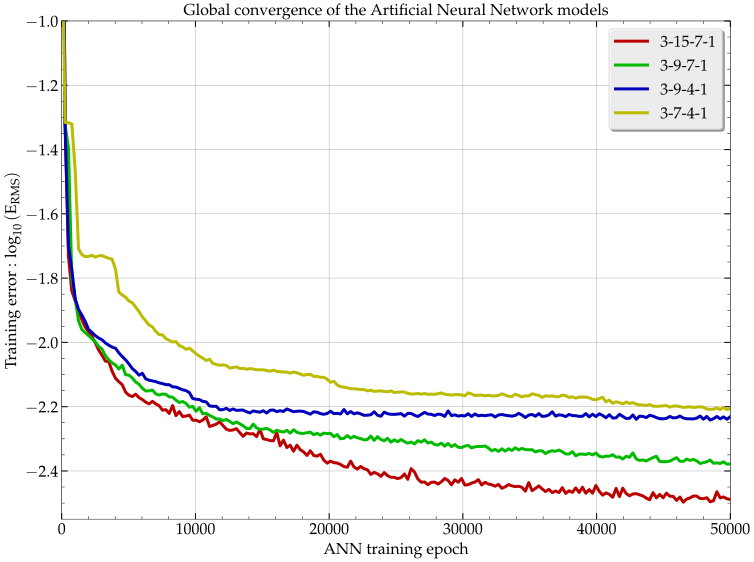
\includegraphics[width=0.9\columnwidth]{Figures/Convergence-ANN}
\caption{Convergence of the ANN models during the training phase.}
\label{fig:Convergence-ANN}
\end{figure}
As we can see on this figure, after $50~000$ iterations, we can consider that we have reached a stationary state of the model learning and that it is useless to continue the learning phase.
As expected, the more neurons the model contains, the more it is able to follow the non-linear evolution of the material's behavior and therefore the more the Mean Square Error ($\MSE$) during the learning phase decreases.
Table \ref{tab:ErrorANN} shows the main results of the training of these neural networks.
\begin{table}[h!]
\centering
\caption{Results concerning the training of the four ANN flow laws.}
\begin{tabular}{lccccc}
	\hline
	ANN    & $n_v$ &  $t$  &    $\MSE$    & $\MARE$ & $\RMSE$ \\
	         &     & (min) & $\times 10^{-5}$ &  (\%)   &  (MPa)  \\ \hline
	3-7-4-1  & 65  &  48   &       3.91       &  1.88   &  3.05   \\
	3-9-4-1  & 81  &  48   &       3.29       &  1.70   &  2.75   \\
	3-9-7-1  & 114 &  49   &       1.83       &  1.25   &  2.44   \\
	3-15-7-1 & 180 &  50   &       1.01       &  0.97   &  2.30\\ \hline
\end{tabular}
\label{tab:ErrorANN}
\end{table}
It can be noted that the number of internal variables $n_v$ of the networks varies from $65$ to $180$ for the most complex and the most powerful one, but that this complexity has no real influence on the learning time $t$ which oscillates around a value of $50$ minutes whatever the architecture chosen.
Concerning the internal accuracy $\MSE$ of the network, it varies in proportions in accordance with the graphical representation of Figure \ref{fig:Convergence-ANN}.

From a more physical point of view, Figure \ref{fig:CompExpANN} shows the correlation between the data predicted by the neural network and the experimental data for the 3-15-7-1 network.
\begin{figure}[!ht]
\centering
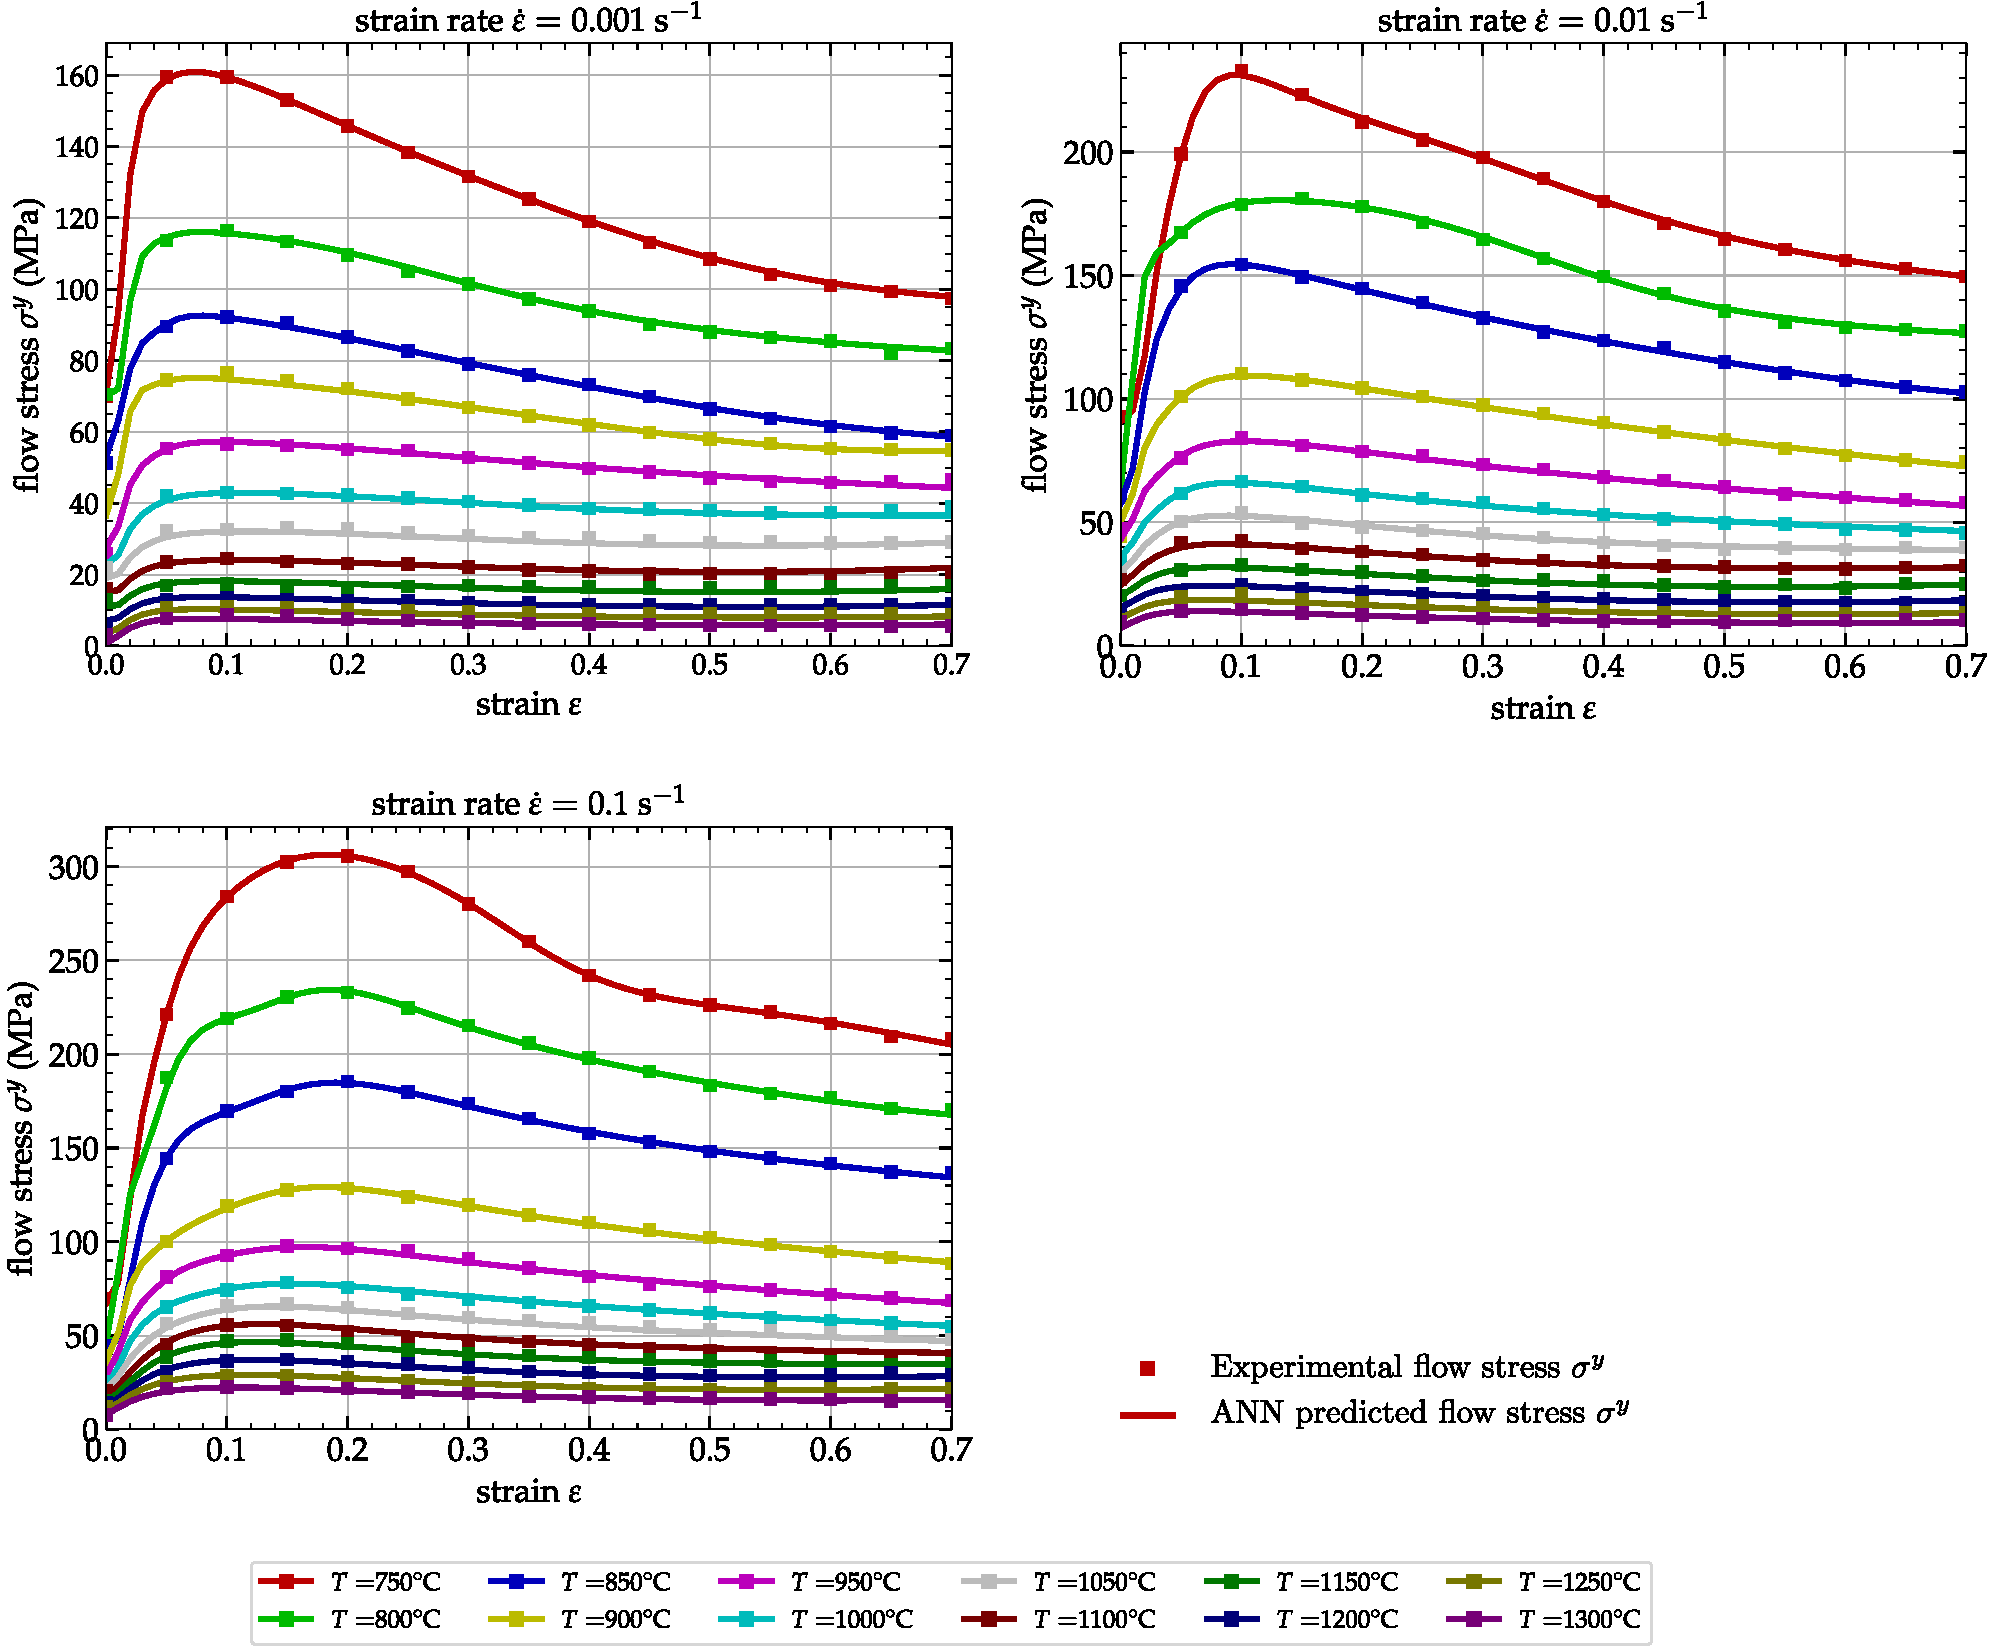
\includegraphics[width=\columnwidth]{Figures/CompExpANN-3-15-7-1}
\caption{Comparison of the flow stress $\sigma^y$ predicted by the 3-15-7-1 ANN and the experimental data for the GCr15.}
\label{fig:CompExpANN}
\end{figure}
There is a very good correlation between the ANN results and the experimental results, which is reflected by the very low values of the $\MARE$ and $\RMSE$ coefficients reported in Table \ref{tab:ErrorANN}.
As reported by Phaniraj \cite{Phaniraj-2003}, the correlation coefficient ($\R$) is generally not a good measure in our case of study because it only shows the correlation of the model with respect to the data and not its accuracy, which is a determining factor in the qualification of a model.
This is why this type of coefficient is not used in this work for comparing the different models.
Concerning the performance of the ANN flow law, the correlation results are much better than the ones obtained by Zhou \eal \cite{Zhou-2020} during his work on the same material with $4$ different flow laws, especially since he was obliged to split the data into two groups according to the temperature value (one on the range $T=750-850~\celsius$ and one on the range $T=850-1300~\celsius$) and to identify two sets of parameters for each flow law in order to reduce the error of his identified analytical models.
This of course raises the question of the usability of those analytical laws in the case where the temperature of the material changes from one group to the other during a thermomechanical transformation.
In our approach and by using an ANN flow law, the identified law is not only valid over the whole temperature range, but it displays an $\MARE$ value $5$ times lower than the best flow law proposed by Zhou \eal \cite{Zhou-2020}: the Arrhenius law with an $\MARE=3.74\%$ over the range $T=750-850~\celsius$ and $\MARE=5.76\%$ over the range $T=850-1300~\celsius$ while the $\MARE=0.97\%$ for the 3-15-7-1 ANN flow law proposed here.

One of the disadvantages of developing a flow law model based on neural networks is the number of internal variables in the network ($180$ in the case of the 3-15-7-1 network), which makes it difficult to translate the network into printable results.
The use of a Johnson-Cook type flow law, for example, allows the reader to quickly get an idea of the law, insofar as the analytical formulation of the law is known to the users, and the behavior of a given material is based on the knowledge of only $5$ internal parameters to be identified, which makes it easy to publish in a table.
Concerning an Arrhenius law, this task becomes a little more complex as one can have from $24$ to $36$ coefficients.
But in our case, the publication of the $180$ coefficients of the model makes this task delicate.
As an illustration, we provide in the Appendix \ref{sec:Appendix} all the coefficients of the 3-15-7-1 model identified during this study.

Once the identification phase has been completed, it is now necessary to transpose this ANN model into a subroutine in FORTRAN or C++ that can be used by a FE code such as Abaqus (for the FORTRAN 77 version) or DynELA (for the C++ version not presented in this paper).
This is the topic of the next Section.

%------------------------------------------------------------------------------------
\section{ANN flow law implementation in FE software}\label{sec:Use}
%------------------------------------------------------------------------------------

Once the neural network has been trained as presented in Section \ref{sec:ANN-traning}, it can be used in a Finite Element code for the numerical simulation of a structure subjected to thermomechanical loading.
This requires the extraction of the internal variables of the neural network and their transfer in the form of a subroutine in FORTRAN 77 based on equations proposed in Sections \ref{sec:ANN-equations} and \ref{sec:ANN-derivative}.

%------------------------------------------------------------------------------------
\subsection{Implementation of the ANN flow law}\label{sec:Implementation}
%------------------------------------------------------------------------------------

If we refer to the general flowchart of a finite element code as shown in Figure \ref{fig:StressUpdate}, the integration of the flow law described by the ANN concerns the computation of the stress tensor $\Sig_1$ at the end of an increment, in the yellow rectangle on the figure.
\begin{figure}[!ht]
\centering
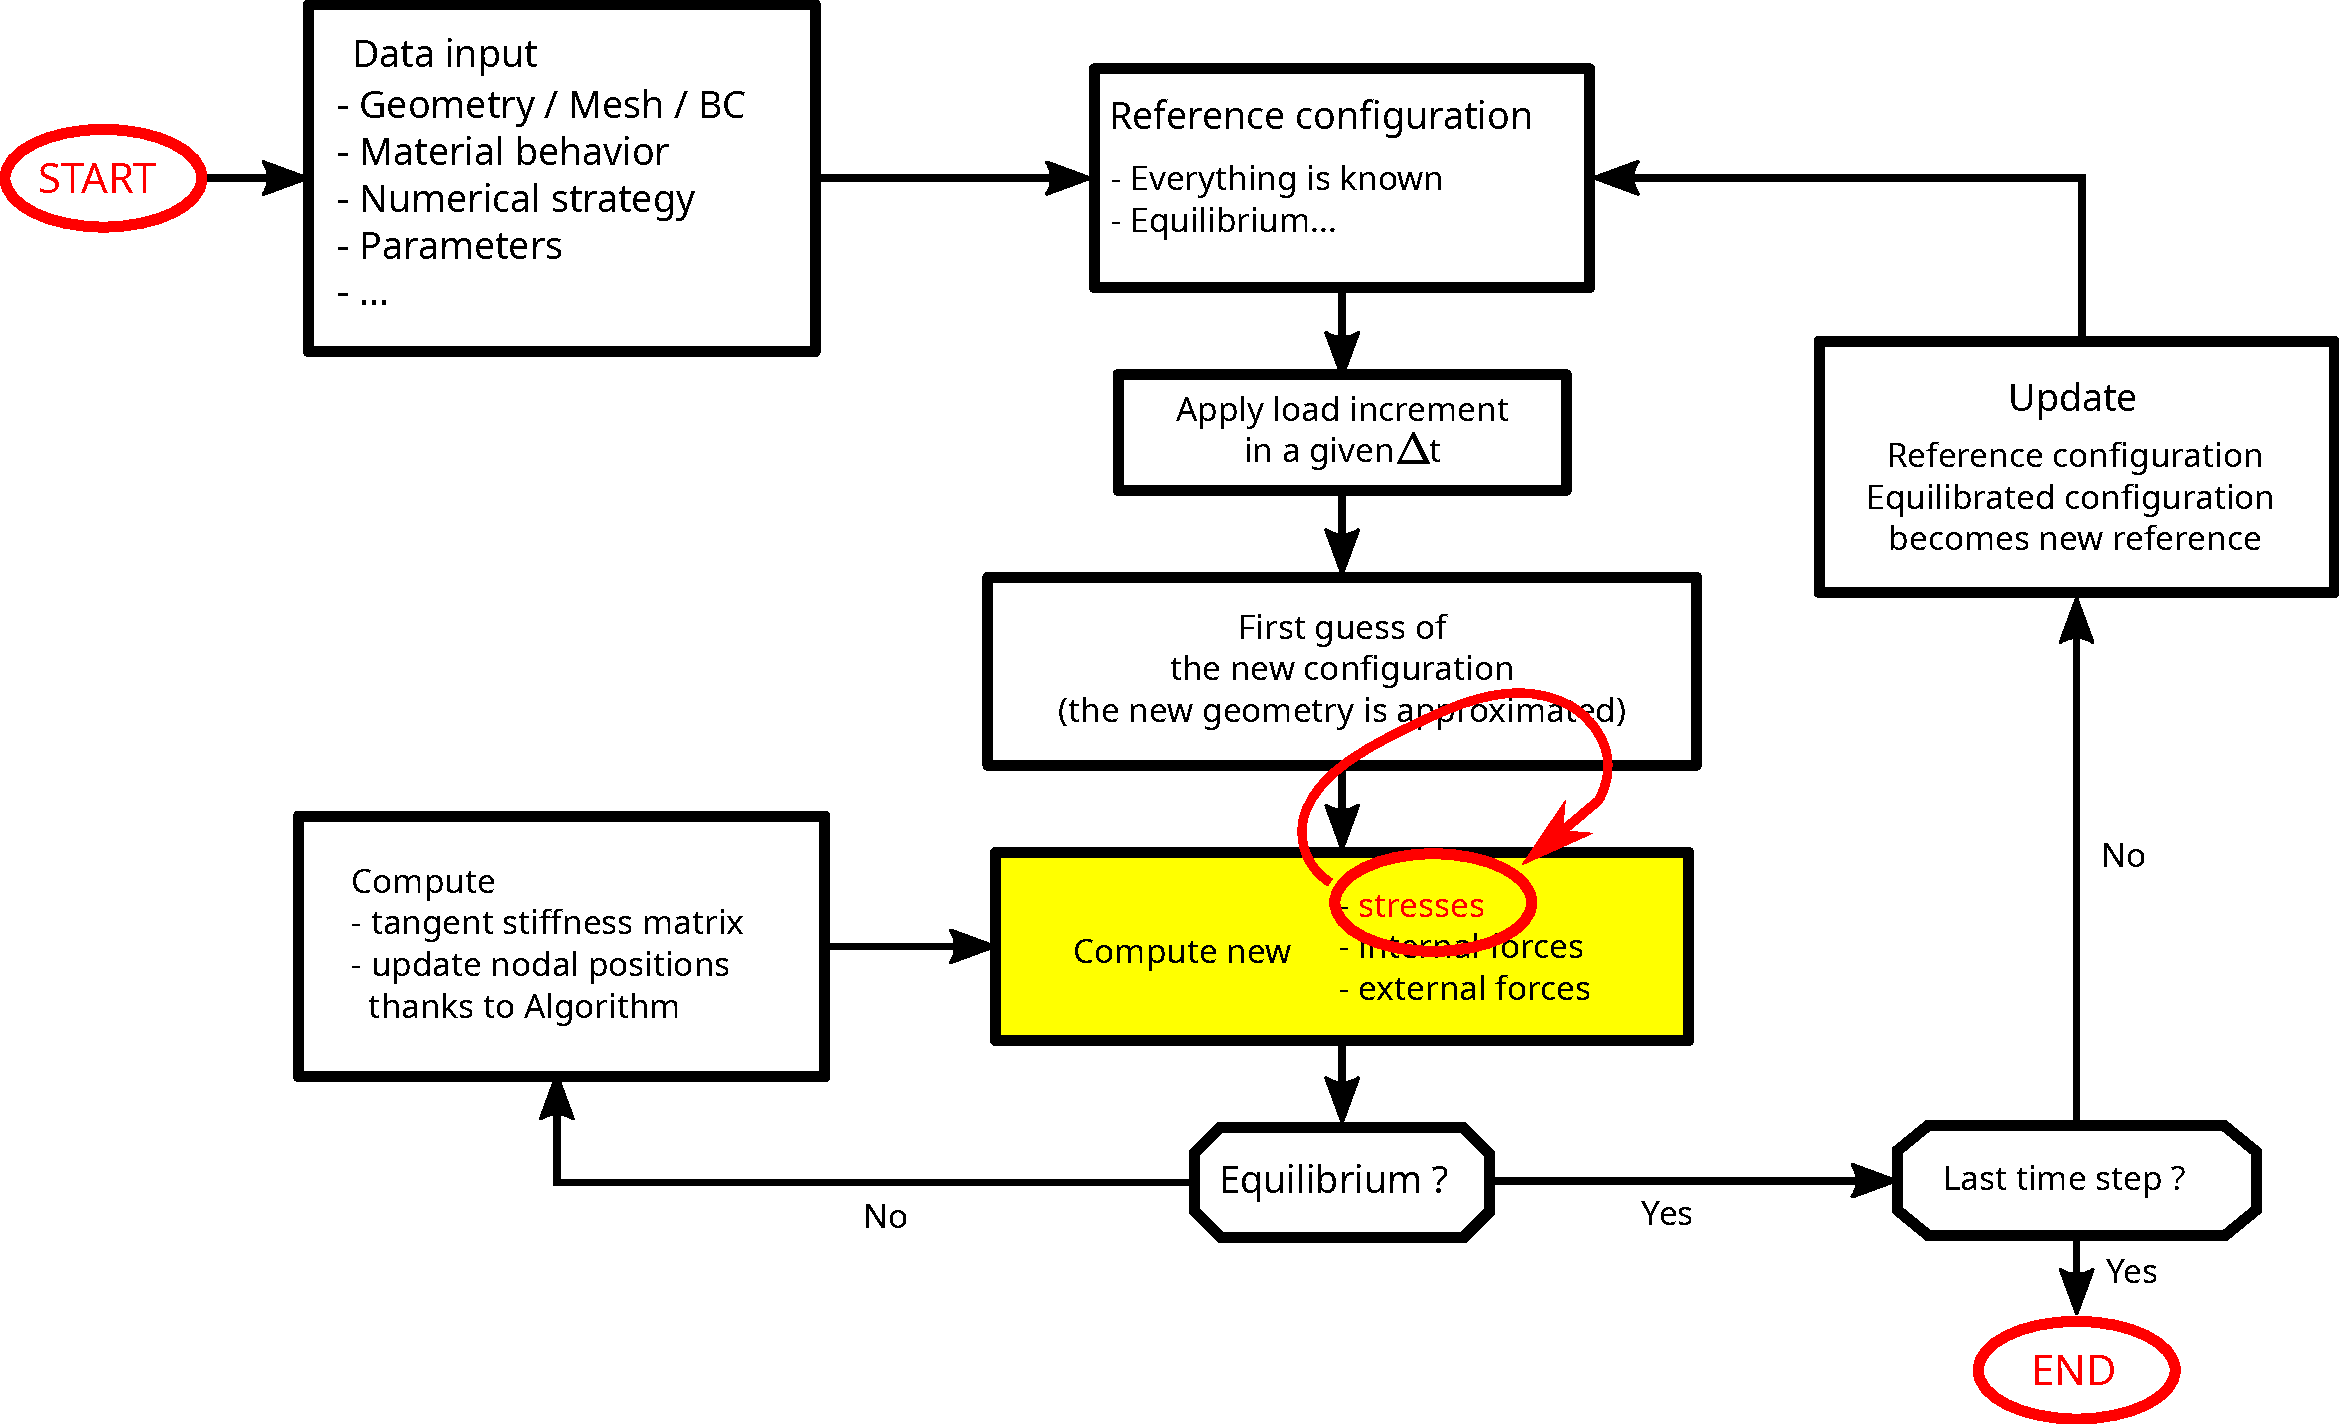
\includegraphics[width=0.9\columnwidth]{Figures/StressUpdate}
\caption{General flowchart of a FE code, focus on the stresses computation.}
\label{fig:StressUpdate}
\end{figure}
Within the framework of a FE formulation in large deformations such as the one used in thermomechanical modeling of processes, this computation of the stress tensor $\Sig_1$ is to be carried out on all the integration points of each element of the studied structure.
Since the numerical model can include thousands of elements, themselves comprising between $1$ and $8$ integration points depending on the nature of the elements used, this stress computation must be as fast as possible in order not to increase the CPU time too much, but precise enough so that the results are in accordance with the physics of the process.
This is even more important if we want to integrate this flow law in an explicit FE code such as Abaqus/Explicit for which one second of physical simulation corresponds to several million iterations of these stress computations.
Thus, the complexity of the ANN, \ie the number of computational steps that must be performed to compute the flow stress as a function of the input variables, is a major parameter in the choice of the neural network.
As an example, for the model presented in section \ref{sec:ANN-traning}, $180$ internal variables, $15$ neurons on the first hidden layer and $7$ neurons on the second hidden layer were listed.
Given the equations described in Sections \ref{sec:ANN-equations} and \ref{sec:ANN-derivative}, it will be necessary to compute $22$ exponentials, to make matrix-vector products of size $15\times3$ and $15\times7$ plus many other numerical operations in order to compute the flow stress $\sigma^y$ and the $3$ derivatives of it with respect to $\varepsilon^p$, $\mdot\varepsilon$ and $T$.

The implementation of the ANN flow law identified above is realized here in a VUHARD subroutine used by the Abaqus Explicit FE code in order to allow a user to program the computation of the flow stress $\sigma^y$ and its 3 derivatives as a function of the model input data.
This subroutine is used when calculating the stress tensor $\Sig_1$ at the end of an increment from the stress tensor at the beginning of the increment $\Sig_0$, the deformations, the material parameters and the history of the deformation at each finite element integration points, according to the stress integration algorithm based on the Radial-Return method as described in Simo \eal \cite{Simo-1998} for the general aspects, Ming \eal \cite{Ming-2018} for Abaqus Explicit FE code or Pantalé \eal \cite{Pantale-2004} for the DynELA FE code.
Thus, without going into too much detail about the stress integration scheme used in finite element codes (the curious reader can refer to \cite{Ponthot-2002, Ming-2018, Pantale-2004, Liang-2022} for details about this method), Figure \ref{fig:RadialReturn} shows the location of the VUHARD subroutine used to compute the flow stress $\sigma^y$ and its derivative $\partial\sigma^y/\partial\Gamma$ used in the writing of the two quantities $\gamma(\Gamma)$ and $\gamma^{'}(\Gamma)$ used in the Newton-Raphson solving procedure from the following relation:
\begin{equation}
\frac{d\sigma^{y}}{d\Gamma} = \sqrt{\frac{2}{3}}\left(\frac{\partial\sigma^{y}}{\partial\varepsilon^{p}}+\frac{1}{\Delta t}\frac{\partial\sigma^{y}}{\partial\mdot{\varepsilon}^p}+\frac{\eta\sigma^{y}}{\rho C_{p}}\frac{\partial\sigma^{y}}{\partial T}\right)\label{eq:derivatives},
\end{equation}
where $\Gamma$ is the consistency parameter used in the Radial-Return algorithm as defined by Simo \eal \cite{Simo-1998}, $\Delta t$ is the time increment, $\eta$ is the Taylor-Quinney coefficient defining the amount of plastic work converted into heat energy, $C_{p}$ is the specific heat coefficient, $\rho$ is the density of the material and $\partial \sigma^y/\partial\varepsilon^p$, $\partial \sigma^y/\partial\mdot\varepsilon$ and $\partial \sigma^y/\partial T$ are the three derivatives defined in Equation (\ref{eq:DANN3}).
\begin{figure}[!ht]
\centering
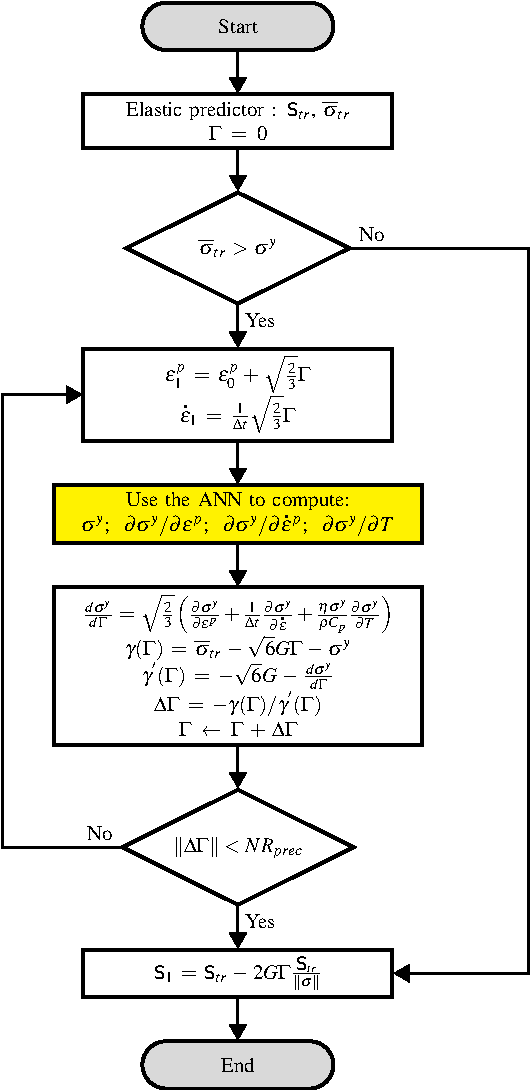
\includegraphics[width=0.6\columnwidth]{Figures/VumatGeneralNewtonRaphson}
\caption{General flowchart of the Radial-Return algorithm to compute the final stress tensor $\Sig_1$.}
\label{fig:RadialReturn}
\end{figure}

%------------------------------------------------------------------------------------
\subsection{Numerical simulations and benchmarks tests}\label{sec:Simulations}
%------------------------------------------------------------------------------------

In order to validate the proposed approach and to compare the different neural network architectures proposed in section \ref{sec:ANN-traning}, we propose here to simulate on the Abaqus Explicit FE code the high-temperature compression of a cylinder on a Gleeble-type thermomechanical device.
We consider a cylinder in compression with an initial diameter $d_0=8~\text{mm}$ and an initial height $h_0=12~\text{mm}$ made of GCr15 material, for which the final height after compression is $h=6~\text{mm}$, that is a reduction of $50\%$ of its total height.
The compression of the sample is done in $10~\text{s}$ so that the strain rate  $\mdot\varepsilon$ is in the corresponding range of the characterization of the material behavior defined by Ji \eal \cite{Ji-2018}.
Concerning the flow laws, the 4 models presented in Section \ref{sec:ANN-traning} will be used and compared between them.
Unfortunately, it is not possible here to compare these results with experimental results, even if the initial shape of the specimen is the same, as these are not available in the references of the work of Zhou \eal \cite{Zhou-2020} or Ji \eal \cite{Ji-2018}.

The mesh of the sample is made with $850$ axisymmetric quadrilateral finite elements with $4$ nodes and reduced integration (named CAX4R in the Abaqus software) with $50$ elements in the vertical direction and $17$ elements in the radial direction respectively.
The cylinder is between two rigid surfaces and a Coulomb friction law with a friction coefficient at the contact surfaces was set to $\mu=0.15$.
The simulation time being fixed at $10~\text{s}$, in order to reduce the simulation time, considering that an explicit integration scheme is used, a global mass scaling is used for all simulations.

Figure \ref{fig:peeqContourplot} shows the plastic strain field $\varepsilon^p$ contourplot within the structure at the end of the simulation for the 3-15-7-1 flow law, while Figure \ref{fig:dpeeqContourplot} shows the plastic strain rate field $\mdot\varepsilon$ contourplot for the same model.
\begin{figure}[!ht]
\centering
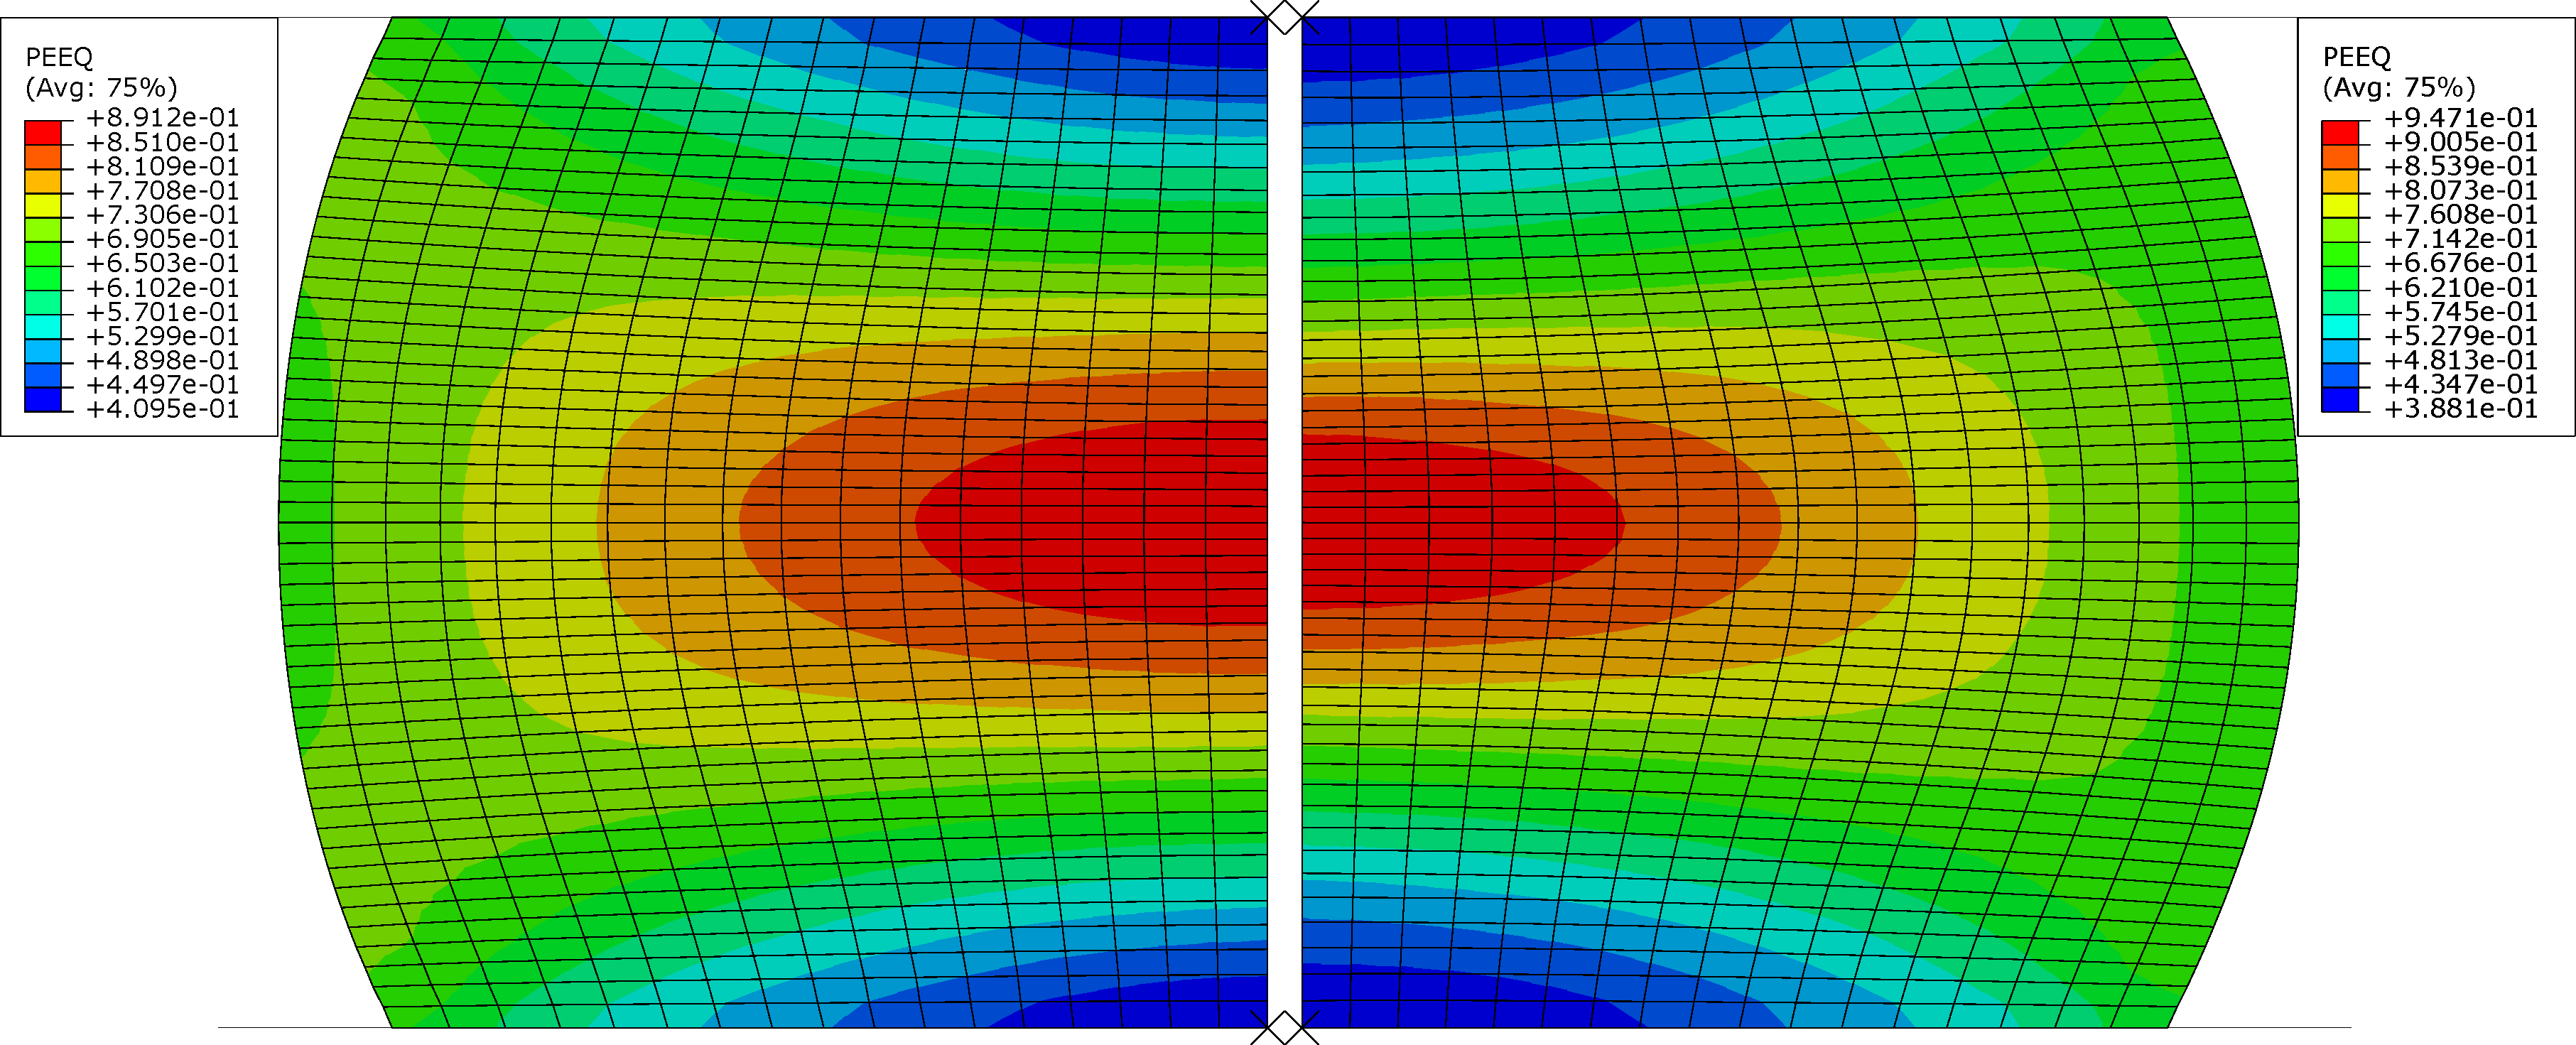
\includegraphics[width=0.60\columnwidth]{Figures/peeq}
\caption{Equivalent plastic strain $\varepsilon^p$ contourplot for the compression of a cylinder using the 3-15-7-1 ANN flow law.}
\label{fig:peeqContourplot}
\end{figure}
\begin{figure}[!ht]
\centering
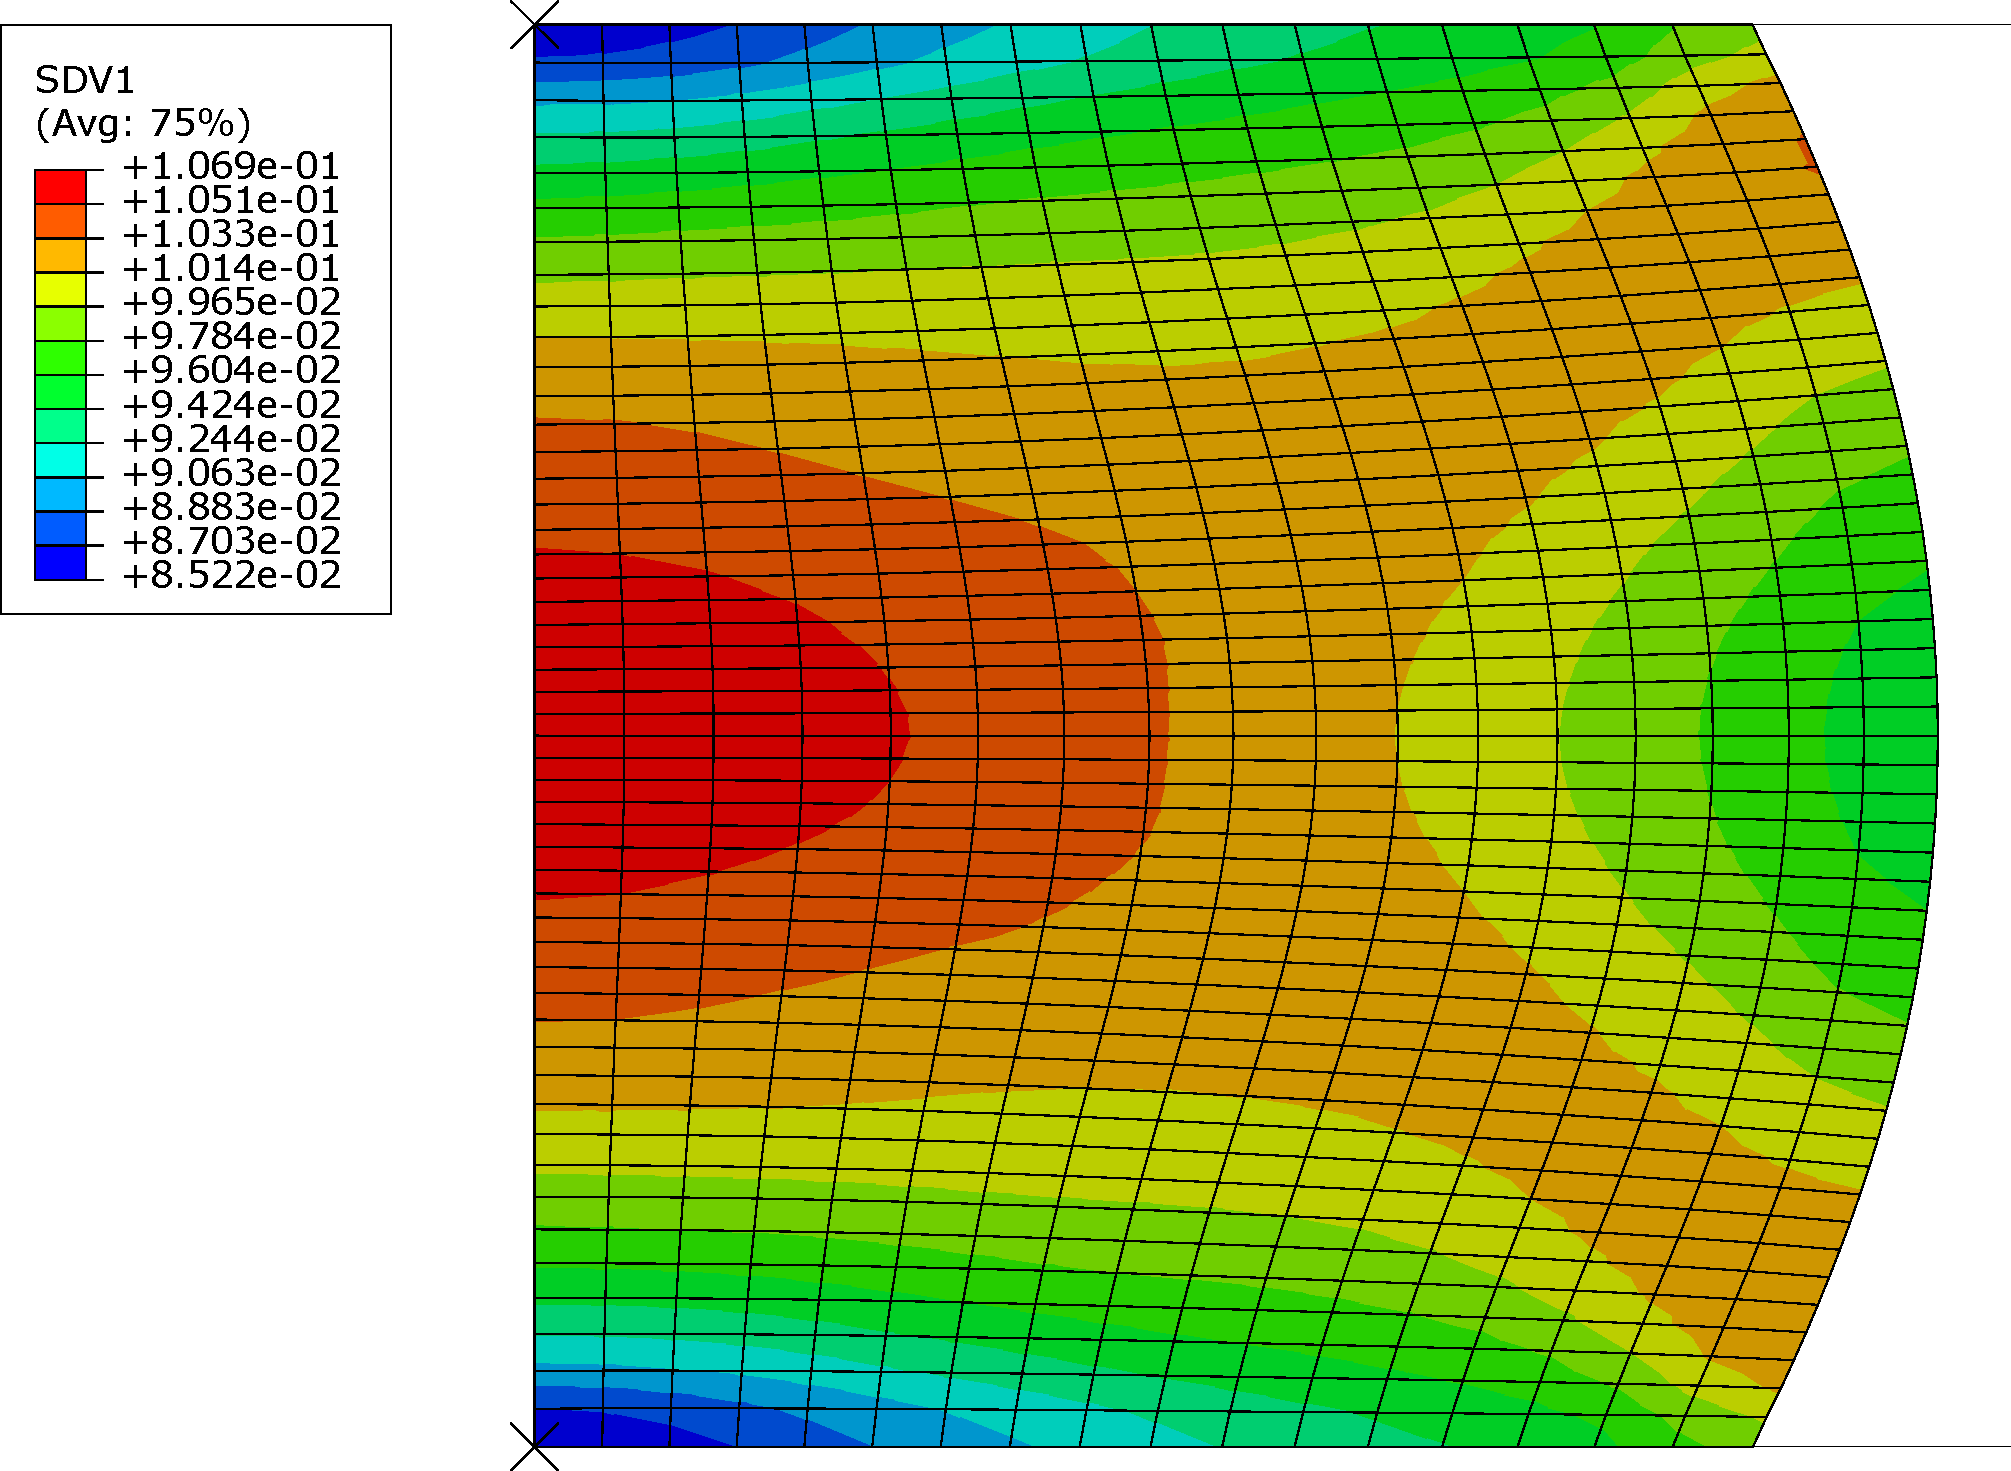
\includegraphics[width=0.60\columnwidth]{Figures/sdv1}
\caption{Equivalent plastic strain rate $\mdot\varepsilon$ contourplot for the compression of a cylinder using the 3-15-7-1 ANN flow law.}
\label{fig:dpeeqContourplot}
\end{figure}
The maximum plastic strains are concentrated in the center of the specimen with a maximum value of $\varepsilon^p=0.947$, which is slightly beyond the limit set by the training data which varies from $0$ to $0.7$.
Nevertheless, as shown by Pantalé \eal \cite{Pantale-2021}, the flow laws defined by neural networks are able to correctly extrapolate the flow stresses $\sigma^y$ when the plastic deformations are higher than at least $150\%$ of the maximum plastic strain used during training.
Concerning the plastic strain rate $\mdot\varepsilon$, the maximum value is around $\mdot\varepsilon=0.1~\ps$, which is in accordance to the experiments used for the learning phase.

Figure \ref{fig:radiusCurve} shows the evolution of the maximum radius $r$ of the cylinder (measured at the middle of the sample height) as a function of the vertical displacement.
\begin{figure}[!ht]
\centering
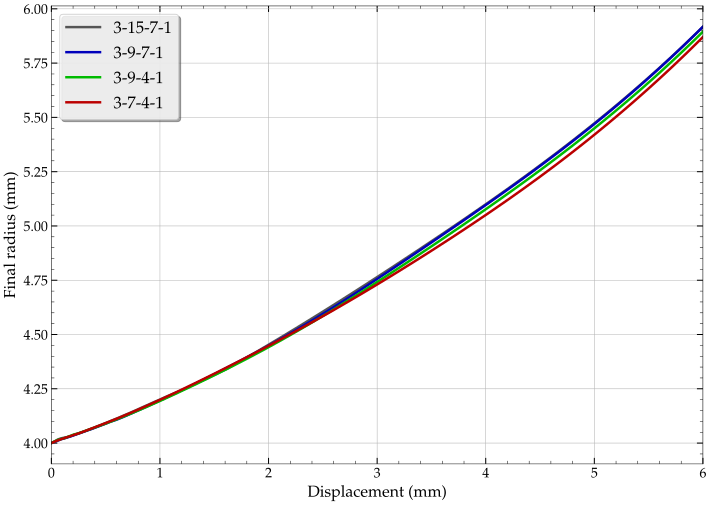
\includegraphics[width=0.75\columnwidth]{Figures/radiusCurve}
\caption{Evolution of the external radius $r$ of the specimen during the compression process using the four ANN flow laws.}
\label{fig:radiusCurve}
\end{figure}
This figure shows a perfect match of the four flow models during the numerical simulation.

Table \ref{tab:SimuResults}, gathers the results allowing the comparison of the four identified flow laws.
It appears from the study of this table that the modification of the number of neurons in the hidden layers has an influence only on the computation time $t$ which increases with the complexity of the network structure as expected and varies within the rage from $944$~s to $1016$~s approximately, since this information is hard to capture from a commercial software that does not contain accurate CPU time reports as the Abaqus software.
Since we have the exact same number of increments $N_{inc}$ for the explicit solver for all four flow laws this increase in the computing time can be directly related to the increase in the complexity of the ANN flow law.
\begin{table}[h!]
\centering
\caption{Compression of a cylinder using the four ANN flow laws, results for the center element of the structure.}
\begin{tabular}{lccccc}
	\hline
	ANN      &  $N_{inc}$  & $t$  &  $r$   & $\varepsilon^p$ &    $T$     \\
	         &         & (s)  &  (mm)  &                 & (\celsius) \\ \hline
	3-7-4-1  & 1418434 & 944  & 5.917 &      0.968      &   796.39   \\
	3-9-4-1  & 1418434 & 962  & 5.917 &      0.968      &   796.39   \\
	3-9-7-1  & 1418434 & 1009 & 5.917 &      0.968      &   796.39   \\
	3-15-7-1 & 1418434 & 1016 & 5.917 &      0.968      &   796.39   \\ \hline
\end{tabular}
\label{tab:SimuResults}
\end{table}
On the other hand, the results, both from the point of view of the dimensional characteristics of the sample (maximum radius $r$), or the internal fields such as the temperatures $T$ and the plastic strains $\varepsilon^p$ in the center of the sample are identical for the four flow models.
There is not any difference between the four models except the computing time, therefore we can conclude that all results agree and are independent of the complexity of the ANN flow law identified.
We can use any of the four formulations in this case.

%------------------------------------------------------------------------------------
\section{Conclusions and future work}\label{sec:Conclusions}
%------------------------------------------------------------------------------------

In this paper, a flow law based on an artificial neural network capable of predicting the flow stress of a material as a function of input data such as strain $\varepsilon$, strain rate $\mdot\varepsilon$ and temperature $T$ for a metallic material subjected to high thermomechanical loading has been presented.

From the equations that govern the writing of the neural network, the expressions of the derivatives of the flow stress of the model as a function of the plastic strain $\varepsilon^p$, the strain rate $\mdot\varepsilon$ and the temperature $T$ have been established.
These expressions allow the transfer of the neural network behavior into a VUHARD subroutine written in FORTRAN 77 language in order to allow the use of this network for the computation of the material flow stresses within the Abaqus FE code.

In a first step, data from the works of Ji \eal \cite{Ji-2018} and Zhou \eal \cite{Zhou-2020}, allowed to train several architectures of the proposed model and to compare the results of these ANN models regarding the fidelity of reproduction of the experimental behavior.
The comparison of the results obtained allowed to validate the approach and to show the superiority of the ANN model compared to the analytical models based on Johnson-Cook or Arrhenius flow laws, both in terms of fidelity of the model and quality of the results.
In a second step, after transferring the training data to the VUHARD subroutines for the Abaqus FE code, we have shown the consistency and quality of the numerical results obtained during the numerical simulation of the compression of a GCr15 alloy cylinder.

This work has thus allowed to highlight the significant contributions of flow laws based on neural networks in the context of numerical simulation by finite elements on a commercial FE code such as the Abaqus software.
The quality of the results obtained allows us to go further in the use of the simulation results and in particular to consider that the results of these finite element simulations can be used to predict the phase transformations and the dynamic recrystallization within the material during the thermomechanical transformation at high temperature.

\vspace{6pt}

%\authorcontributions{For research articles with several authors, a short paragraph specifying their individual contributions must be provided. The following statements should be used ``Conceptualization, X.X. and Y.Y.; methodology, X.X.; software, X.X.; validation, X.X., Y.Y. and Z.Z.; formal analysis, X.X.; investigation, X.X.; resources, X.X.; data curation, X.X.; writing---original draft preparation, X.X.; writing---review and editing, X.X.; visualization, X.X.; supervision, X.X.; project administration, X.X.; funding acquisition, Y.Y. All authors have read and agreed to the published version of the manuscript.'', please turn to the  \href{http://img.mdpi.org/data/contributor-role-instruction.pdf}{CRediT taxonomy} for the term explanation. Authorship must be limited to those who have contributed substantially to the work~reported.}

\funding{This research received no external funding.}

%\institutionalreview{In this section, you should add the Institutional Review Board Statement and approval number, if relevant to your study. You might choose to exclude this statement if the study did not require ethical approval. Please note that the Editorial Office might ask you for further information. Please add “The study was conducted in accordance with the Declaration of Helsinki, and approved by the Institutional Review Board (or Ethics Committee) of NAME OF INSTITUTE (protocol code XXX and date of approval).” for studies involving humans. OR “The animal study protocol was approved by the Institutional Review Board (or Ethics Committee) of NAME OF INSTITUTE (protocol code XXX and date of approval).” for studies involving animals. OR “Ethical review and approval were waived for this study due to REASON (please provide a detailed justification).” OR “Not applicable” for studies not involving humans or animals.}

%\informedconsent{Any research article describing a study involving humans should contain this statement. Please add ``Informed consent was obtained from all subjects involved in the study.'' OR ``Patient consent was waived due to REASON (please provide a detailed justification).'' OR ``Not applicable'' for studies not involving humans. You might also choose to exclude this statement if the study did not involve humans.

%Written informed consent for publication must be obtained from participating patients who can be identified (including by the patients themselves). Please state ``Written informed consent has been obtained from the patient(s) to publish this paper'' if applicable.}

\dataavailability{Source files of the numerical simulations are available from the author.}

%\acknowledgments{In this section you can acknowledge any support given which is not covered by the author contribution or funding sections. This may include administrative and technical support, or donations in kind (e.g., materials used for experiments).}

\conflictsofinterest{The authors declare no conflict of interest.}

%\sampleavailability{Samples of the compounds ... are available from the authors.}

%% Only for journal Encyclopedia
%\entrylink{The Link to this entry published on the encyclopedia platform.}

\abbreviations{Abbreviations}{
The following abbreviations are used in this manuscript:\\

\noindent
\begin{tabular}{@{}ll}
	ANN & Artificial Neural Network \\
	DRX & Dynamic Recrystallization \\
	CPU & Central Processing Unit   \\
	FE  & Finite Element\\
	VUMAT & User subroutine to compute the stress tensor for Abaqus/Explicit\\
	VUHARD & User subroutine to compute the flow stress for Abaqus/Explicit
\end{tabular}
}


\appendixtitles{no} % Leave argument "no" if all appendix headings stay EMPTY (then no dot is printed after "Appendix A"). If the appendix sections contain a heading then change the argument to "yes".
\appendixstart
\appendix
%----------------------------------------------------------------------------------
\section[\appendixname~\thesection]{ANN flow law coefficients\label{sec:Appendix}}
%----------------------------------------------------------------------------------

In order to complete this paper, we report here after the computing process and the $180$ coefficients of the Artificial Neural Network ANN-3-15-7-1 model used in Section \ref{sec:ANN-traning}.
The weight matrix for the first hidden layer $\w_1$ is a $15\times3$ matrix:
\begin{equation*}
\w_1 = \left[
\begin{array}{rrr}
1.9555 & -1.4358 & 3.8147\\
-3.7376 & 2.5796 & -63.8787\\
-1.0201 & 0.4169 & -7.6105\\
4.7550 & -8.2280 & -39.1221\\
-4.4573 & 1.6931 & -16.1442\\
-7.4413 & 4.9264 & -10.9690\\
-0.0151 & -0.3780 & -43.0122\\
0.7121 & 0.6326 & -3.0630\\
-2.9821 & -1.0429 & -8.6435\\
0.7087 & 3.3178 & -22.7078\\
-1.1669 & -7.5672 & -8.5390\\
-46.2443 & -0.0546 & -2.2126\\
-5.1689 & -1.1643 & -5.3561\\
3.2716 & 2.5842 & -8.8036\\
-14.9815 & 3.7360 & -4.4927\\
\end{array}\right]
\end{equation*}
The biases of the first hidden layer $\overrightarrow{b_1}$ is a $15$ components vector:
\begin{equation*}
\overrightarrow{b}_1 = \left[
\begin{array}{r}
-1.9351\\
-0.7234\\
1.0962\\
5.5862\\
0.9015\\
-1.7936\\
4.5917\\
-0.7919\\
0.1110\\
-1.4496\\
0.5536\\
0.0852\\
0.7880\\
1.4652\\
-1.8652\\
\end{array}\right]
\end{equation*}
The weight matrix for the second hidden layer $\w_2$ is a $7\times15$ matrix:
\begin{equation*}
\w_2^T = \left[
\begin{array}{rrrrrrr}
1.3033 & -6.6636 & -1.1191 & 0.0640 & -1.2000 & -0.7778 & -0.0832\\
3.4156 & -1.9712 & 1.1247 & 11.3150 & -5.3441 & 2.6273 & -7.4426\\
0.6366 & -1.5008 & 0.3228 & -3.6627 & 1.1657 & -0.4301 & -2.1017\\
2.7161 & 1.8167 & 3.1051 & 3.3271 & 3.1566 & -3.7084 & -0.0561\\
3.2426 & 0.5226 & 1.0579 & -4.6344 & -4.8619 & 1.8223 & -0.6718\\
-2.0943 & 2.4590 & -1.0508 & 4.5012 & 6.6691 & 2.7379 & -3.2888\\
-5.2160 & -3.2763 & -0.7033 & -1.1473 & 3.9384 & -0.9496 & -0.5450\\
-3.7103 & -0.3289 & 0.5146 & -0.8302 & -1.6758 & 2.1605 & 0.5720\\
0.0661 & 0.6169 & 0.5066 & -5.5835 & -2.0816 & 0.0687 & -3.8897\\
-0.8534 & 5.1127 & -0.4439 & 2.7771 & -2.8935 & 0.8596 & -3.8329\\
-2.7441 & -1.8542 & -5.3622 & -1.9153 & -0.6710 & 1.2238 & 1.3638\\
13.2086 & -21.6848 & 1.9939 & 6.0605 & 4.1271 & 12.2979 & -3.0547\\
1.3170 & 2.2413 & -0.8415 & -1.1919 & 1.0253 & 0.4586 & 2.4214\\
-1.3138 & -2.2316 & 0.6675 & 0.5940 & 1.3283 & -1.8264 & -0.1424\\
3.4473 & -1.1443 & -0.4509 & 12.7328 & 4.0328 & -0.4105 & -0.1603\\
\end{array}\right]
\end{equation*}
The biases of the second hidden layer $\overrightarrow{b_2}$ is a 7 components vector:
\begin{equation*}
\overrightarrow{b}_2 = \left[
\begin{array}{r}
-1.8551\\
-0.7994\\
-0.8867\\
0.5204\\
-3.4375\\
-0.7264\\
-0.4300\\
\end{array}\right]
\end{equation*}
The weight vector for the output layer $\overrightarrow{w}$ is a 7 components vector:
\begin{equation*}
\overrightarrow{w} = \left[
\begin{array}{r}
-0.4036\\
1.9957\\
0.3469\\
-0.1811\\
-0.1828\\
0.2522\\
-0.8099\\
\end{array}\right]
\end{equation*}
The bias of the output layer $b$ is a scalar:
\begin{equation*}
b = 0.4699
\end{equation*}

The boundaries of the range of the corresponding field are:
\begin{itemize}
\item $\varepsilon^p\!\in\!\left[0.0,0.7\right]$
\item $\mdot{\varepsilon}\!\in\!\left[0.001~\ps,0.1~\ps\right]$
\item $T\!\in\!\left[750~\celsius,1300~\celsius\right]$
\item $\sigma\!\in\!\left[3.052~\MPa,306.0956~\MPa\right]$.
\end{itemize}
The reference strain rate is $\mdot{\varepsilon_0} = 0.001~\ps$.

\reftitle{References}

% Citations and References in Supplementary files are permitted provided that they also appear in the reference list here.

%=====================================
% References, variant A: external bibliography
%=====================================
\bibliography{bibliography}




% If authors have biography, please use the format below
%\section*{Short Biography of Authors}
%\bio
%{\raisebox{-0.35cm}{\includegraphics[width=3.5cm,height=5.3cm,clip,keepaspectratio]{Definitions/author1.pdf}}}
%{\textbf{Firstname Lastname} Biography of first author}
%
%\bio
%{\raisebox{-0.35cm}{\includegraphics[width=3.5cm,height=5.3cm,clip,keepaspectratio]{Definitions/author2.jpg}}}
%{\textbf{Firstname Lastname} Biography of second author}

% For the MDPI journals use author-date citation, please follow the formatting guidelines on http://www.mdpi.com/authors/references
% To cite two works by the same author: \citeauthor{ref-journal-1a} (\citeyear{ref-journal-1a}, \citeyear{ref-journal-1b}). This produces: Whittaker (1967, 1975)
% To cite two works by the same author with specific pages: \citeauthor{ref-journal-3a} (\citeyear{ref-journal-3a}, p. 328; \citeyear{ref-journal-3b}, p.475). This produces: Wong (1999, p. 328; 2000, p. 475)

%%%%%%%%%%%%%%%%%%%%%%%%%%%%%%%%%%%%%%%%%%
%% for journal Sci
%\reviewreports{\\
%Reviewer 1 comments and authors’ response\\
%Reviewer 2 comments and authors’ response\\
%Reviewer 3 comments and authors’ response
%}
%%%%%%%%%%%%%%%%%%%%%%%%%%%%%%%%%%%%%%%%%%
%\end{adjustwidth}
\end{document}

